%Documento elaborado através da modificação de Template_ Tese_ MAEG por RJF. 
%Com contribuições e modificações dos alunos do DEGGE e Phd student 
%Angelo Soares (arsoares@fc.ul.pt) com orientação de Carla M. Silva.
%11/11/2021
% Para escrever neste documento, expandam a secção Capitulos e escrevam no capitulo apropriado.
% Após a escrita, seleccionem "main.tex" e recompilem. Tudo o que escreverem nos capitulos irá 
% aparecer. 

% ------------------------------------------------------------------------------------------------------%
% ------------------------------------------ ALTERAR CAPA ----------------------------------------------%
% ------------------------------------------------------------------------------------------------------%
%A Neste main.tex as únicas alterações que precisam de fazer são referentes à Capa da
%dissertação. Sigam as indicações seguintes: Façam ctrl+F para procurar "includepdf" e leiam 
%as notas por baixo do \includepdf.

% ------------------------------------------------------------------------------------------------------%

%Outras Notas: 
%1. Ler o conteudo em "library.bib".
%2. O GOOGLE é vosso amigo, todas e quaisquer modificações necessárias, seja para introduzir um
%certo tipo de formatação, seja para colocar uma figura ou tabela com especificações particulares,
%usem o GOOGLE, existem N exemplos para todo o tipo de alteração em latex. Com quase copy+paste
%code.
% ------------------------------------------ IMPORTANTE -----------------------------------------------%
%3. Neste documento existem algumas colisoes de pacotes, nomeadamente o tocloft e o book report
%e a maneira %como o chapter foi elaborado. Exemplo: Se os alunos quiserem colocar o prefixo "1."
%antes da introdução, ou seja "1. Introdução". No Indice ficaria "1 1. Introdução".
%ALTERNATIVA: Escrevam a dissertação na totalidade. No fim, façam download do PDF (cliquem segundo
%Icone após o Recompile). Com esse ficheiro PDF, abram-no no PDF reader (adobe acrobat pro) e 
%editem acrescentando o número do capitulo para ficar igual ao que está no Indice "1. Introdução".
%É a forma mais simples de resolver.

%Se alguem por curiosidade encontrar outra solução usando o tocloft package, como por exemplo, 
%ocultar o número do capitulo no TOC sem usar \chapter* ou interferir com o hyperref enviem essa
%info para o email supramencionado, muito obrigado.
%Boa sorte


\documentclass[11pt,a4paper,twoside,openright]{book}
% ------------------------------------------------------------------------------------------------------%
% ------------------------------------------- PREAMBLE -------------------------------------------------%
% ------------------------------------------------------------------------------------------------------%
\usepackage{mathptmx} % Fonte mais próxima de Times New Roman
% Alterar margens do documento
\usepackage[margin=2.5cm]{geometry}
\renewcommand{\baselinestretch}{1.15}
\usepackage{setspace}
\usepackage{fancyhdr}
\usepackage{pgfplots}
\pagestyle{fancy}
\renewcommand{\chaptermark}[1]{\markboth{\MakeUppercase{\thechapter. #1 }}{}}
\renewcommand{\sectionmark}[1]{\markright{\thesection\ #1}}
\fancyhf{}
\fancyhead[RO]{\small{\rightmark}}
\fancyhead[LE]{\small{\leftmark}}
\setlength{\headheight}{12pt}
\addtolength{\topmargin}{-10.5pt}
\fancyfoot[C]{\thepage}
\renewcommand{\headrulewidth}{0pt}
\renewcommand{\footrulewidth}{0pt}
\addtolength{\headheight}{0.5pt}
\fancypagestyle{plain}{
  \fancyhead{}
  \renewcommand{\headrulewidth}{0pt}
}
\usepackage[utf8]{inputenc}
\usepackage{neuralnetwork}
\usepackage{datatool}
\usepackage{mathtools}
\usepackage[backend=biber, natbib=true, style=numeric-comp, sorting=none]{biblatex} %Numeric style
%\usepackage[backend=biber,style=authoryear,maxcitenames=1,autocite=inline,natbib=true]{biblatex}
%\addbibresource{library} %O ficheiro .bib que a bibliografia vai usar
%\bibliography{library}
%\addbibresource{library.bib} %O ficheiro .bib que a bibliografia vai usar
%\bibliography{library}
\addbibresource{library.bib}


\usepackage{tikz}
    \usetikzlibrary{positioning, calc}
	\usetikzlibrary{fit}
	\usetikzlibrary{matrix, arrows}
 \usepgflibrary{shapes.misc} 
\tikzset{basic/.style={draw,fill=none,
                       text badly centered,minimum width=1.5em}}
\tikzset{input/.style={basic,circle,minimum width=1.75em}}
\tikzset{small_input/.style={basic,circle,minimum width=0.4em}}
\tikzset{weights/.style={basic,rectangle,minimum width=1em}}
\tikzset{neurons/.style={basic,rectangle,minimum width=1em, dashed}}
\tikzset{functions/.style={basic,circle, minimum width=2em}}
\newcommand{\addaxes}{\draw (0em,0.5em) -- (0em,-0.5em)
                            (-0.5em,0em) -- (0.5em,0em);}
\newcommand{\relu}{\draw[line width=0.75pt] (-0.5em,0) -- (0,0)
                                (0,0) -- (0.375em,0.375em);}
\newcommand{\stepfunc}{\draw[line width=0.75pt] (0.325em,0.325em) -- (0,0.325em) 
                                    -- (0,-0.325em) -- (-0.325em,-0.325em);}
%\bibliographystyle XXX
%\usepackage[numbers]{natbib}1
\usepackage{nicematrix}
% Package que permite incluir imagens
\usepackage{graphicx}
% Comentar para não incluir a lista de figuras e tabelas no índice
\usepackage[nottoc]{tocbibind}

% Para citar referências
%\usepackage{natbib}
%\setcitestyle{numbers}
%\bibliographystyle{humannat}
%\setcitestyle{authoryear}

%Indentar primeiro parágrafo
\usepackage{indentfirst}

% Incluir até à subsecção no índice
\setcounter{tocdepth}{3}
\setcounter{secnumdepth}{3}

% Permite remover os espaços entre itens
\usepackage{enumitem}

% Caption para imagens
\usepackage[font=footnotesize]{caption}

% Referenciar anexos
\usepackage[toc,page]{appendix}

%Adicionar pdfs
\usepackage{pdfpages}

%Alterar nome de capitulo para a referencia
\usepackage{fmtcount}
\usepackage{url}

%Para expressões Matemáticas
\usepackage{amsmath}
\usepackage{bm}

%Bibliotecas
%\usepackage{biblatex}
%\usepackage[portugues]{babel} %Can be switched to english
%\usepackage{csvsimple}
\usepackage{csvsimple-l3}
\usepackage{float}
\raggedbottom
\usepackage{subcaption}
\usepackage{eurosym}
\usepackage{booktabs}
\usepackage[T1]{fontenc}
\usepackage{csquotes}
\usepackage{tabularx}
%\usepackage[scaled]{helvet}
%\renewcommand*\familydefault{\sfdefault}

%Comando que cria abreviaturas usado no Nomenclatura
\newcommand{\abbreviations}[1]{%
\vspace{12pt}\noindent{\selectfont\textbf{Abreviaturas}\par\vspace{6pt}\noindent {\fontsize{9}{9}\selectfont #1}\par}}
%Criar Siglas
\newcommand{\siglas}[1]{%
\vspace{12pt}\noindent{\selectfont\textbf{Siglas e acrónimos}\par\vspace{6pt}\noindent {\fontsize{9}{9}\selectfont #1}\par}}
%Cria simbologia
\newcommand{\simbolos}[1]{%
\vspace{12pt}\noindent{\selectfont\textbf{Simbologia}\par\vspace{6pt}\noindent {\fontsize{9}{9}\selectfont #1}\par}}

\makeatletter
\def\cleardoublepage{\clearpage\if@twoside \ifodd\c@page\else
    \hbox{}
    \thispagestyle{plain}
    \newpage
    \if@twocolumn\hbox{}\newpage\fi\fi\fi}
\makeatother \clearpage{\pagestyle{plain}\cleardoublepage}

\providecommand{\keywords}[1]{\textbf{Keywords:} #1}
\providecommand{\keywordsP}[1]{\textbf{Palavras chave:} #1}

%Remover Chapter N on the header
\usepackage{titlesec}
\usepackage{lipsum}
\titleformat{\chapter}[display]
   {\normalfont\huge\bfseries}{\chaptertitlename\ \thechapter}{20pt}{\Huge}   
\titlespacing*{\chapter}{0pt}{-20pt}{40pt}
\titleformat{\chapter}[display]{\normalfont\bfseries}{}{0pt}{\huge}

%\numberwithin{section}{chapter}
\usepackage{multirow}
\usepackage{chngcntr}  
\usepackage{tocloft}
\usepackage[hidelinks]{hyperref}
\hypersetup{
    colorlinks=true,
    linkcolor=black,  % color of internal links
    filecolor=black,  % color of links to local 
      urlcolor=blue,
}
%\counterwithout{figure}{chapter}
%\counterwithout{table}{chapter}

\renewcommand{\cftfigpresnum}{\textbf{Figura\ }}
\renewcommand{\cfttabpresnum}{\textbf{Tabela\ }}

\newlength{\mylenf}
\settowidth{\mylenf}{\cftfigpresnum}
\setlength{\cftfignumwidth}{\dimexpr\mylenf+1.5em}
\setlength{\cfttabnumwidth}{\dimexpr\mylenf+1.5em}

\sloppy

\makeatletter
\newcommand\listoftablesandfigures{%
    \chapter*{List of Tables and Figures}%
    \phantomsection
\@starttoc{lof}%
\bigskip
\@starttoc{lot}}
\makeatother

\PassOptionsToPackage{hyphens}{url}\usepackage{hyperref}

% ------------------------------------------------------------------------------------------------------%
% ------------------------------------------- END - PREAMBLE -------------------------------------------%
% ------------------------------------------------------------------------------------------------------%

\begin{document}


% Capa
\newpage
\thispagestyle{empty}

%\setmainfont[Path = fonts/]{arial_narrow.ttf} 

\centering{\fontsize{12.2}{14.4}\selectfont UNIVERSIDADE DE LISBOA}\\
\centering{\fontsize{12.2}{14.4}\selectfont FACULDADE DE CIÊNCIAS}\\
\centering{\fontsize{12.2}{14.4}\selectfont DEPARTAMENTO DE ENGENHARIA GEOGRÁFICA,GEOFÍSICA E ENERGIA}

\vspace{1.3cm}

\begin{figure}[h]
 \centering
 
\includegraphics[width = 6.99cm,height = 3.3cm]{Imagens/logo_fcul.png}
\end{figure}

\vspace{3.45cm}

%\setmainfont[Path = fonts/]{arial_narrow_bold.ttf}

\centering{\fontsize{17}{20.4}\selectfont \textbf{Participação da geração renovável no mercado de reservas de um sistema eléctrico}}

%\setmainfont[Path = fonts/]{arial_narrow.ttf}

\vspace{4cm}

\centering{\fontsize{14}{16.8}\selectfont João Pedro Passagem dos Santos}

\vspace{1.3cm}

%\setmainfont[Path = fonts/]{arial_narrow_bold.ttf}

\centering{\fontsize{13}{15.6}\selectfont \textbf{Mestrado em Engenharia da Energia e Ambiente}}\\

%\setmainfont[Path = fonts/]{arial_narrow.ttf}

%\centering{\fontsize{13}{15.6}\selectfont Especialização em Bioinformática}

\vspace{0.5cm}


\vspace{0.5cm}

\centering{\fontsize{13}{15.6}\selectfont Dissertação orientada por:}\\
\centering{\fontsize{13}{15.6}\selectfont Doutor Hugo Algarvio}\\
\centering{\fontsize{13}{15.6}\selectfont Professora Doutora Ana Estanqueiro}\\

\vspace{2.9cm}

\centering{\fontsize{14}{16.8}\selectfont 2023}
\label{Capa}



\let\cleardoublepage\clearpage


\clearpage \thispagestyle{empty}\mbox{}\clearpage

\frontmatter
% RESUMO
\newpage
\thispagestyle{plain}
\chapter{Resumo}
\justifying

A crescente penetração de fontes de energia renováveis variáveis no tempo, vRES, no sistema eléctrico, como a solar ou eólica, está a transformar significativamente os mercados de eletricidade, devido à sua natureza intermitente e imprevisível. Isso torna as previsões de produção e consumo de energia mais desafiantes, especialmente porque os mercados fecham entre 1 e 37 horas antes da entrega real da energia, podendo originar discrepâncias entre as energias contratadas e necessárias. Manter o equilíbrio entre a oferta e a procura em tempo real é vital para a segurança e estabilidade da rede, função que recai principalmente sobre os operadores de redes de transporte (TSO).\par
Os TSO utilizam mercados de reserva de energia, onde adquirem de forma simétrica potência secundária ascendente e descendente, com base em previsões de procura para as horas subsequentes. No entanto, essa abordagem é ineficaz face às flutuações das renováveis, levando à necessidade de ajustes mais dinâmicos e precisos.\par
Este trabalho propõe um estudo de parâmetros fórmula do TSO português para a previsão de reserva necessária ($\rho$), onde, usando os dados históricos horários no período de 2008 a 2023, é calculado o $\rho$ que apresente menor erro na previsão, atingindo erros inferiores a 5\%.\par
O presente trabalho propõe também um modelo \textit{machine learning} para calcular dinamicamente as reservas de potência secundária, utilizando dados operacionais abertos do TSO espanhol. O modelo foi treinado com dados no período de 2014 a 2023, e validado com dados de referência de 2019 a 2022. A metodologia proposta demonstra uma melhoria significativa na utilização das reservas de potência secundária, com um aumento de aproximadamente 47\% na eficiência das reservas ascendentes e cerca de 42\% nas reservas descendentes. Este avanço contribui para uma gestão mais eficiente e equilibrada do sistema elétrico, especialmente em cenários com elevada penetração de vRES.\par




\vspace{0.5cm} %adiciona um espaço de 0.5cm entre o texto e as palavras chave.

\keywordsP{sistemas de reserva, mercados de energia, redes neuronais, previsões}
%reparem que # necessita de um \ para que o latex o interprete correctamente como um caracter especial. Isto também acontece com % por exemplo.
\label{resumo}

%Abstract
\newpage
\thispagestyle{plain}
\chapter{Abstract}
The growing penetration of renewable energy sources, in the energy produtction markets, together with the paradigm shift in size and centralization of producers, brings instabilities and variability not in the scoope of current market models. \\

In turn, due to their less constante nature, these renewble producers have greater difficulties in making a profit in current models. \\

Forecast technologies are increasingly migrating to \emph{machine learning} models, with more accurate results. \\

This work proposes the application of neural network technologies to forecast forecast secondary reserve allocation bands, using data from the Iberian market. \\

\vspace{0.5cm} %adiciona um espaço de 0.5cm entre o texto e as palavras chave.

\keywordsP{reserve systems,energy markets, neural networks, forecast}
%notice that # requires a \ so that latex correctly interprets it as a special character. This also happens with % for example.
\label{abstract}

% AGRADECIMENTOS
\newpage
\thispagestyle{plain}
\chapter{Agradecimentos}
\justifying

Começo por agradecer à minha família, que me acompanhou sempre neste longo e atribulado percurso académico.\par
Agradeço a todos os amigos que me inspiraram e me fizeram crescer pessoal, profissional e academicamente.\par
Um agradecimento especial à Ana, pelo companheirismo, apoio, jantares e trabalho constante de me manter em rumo. \par
Por último agradeço aos meus orientadores, a professora Doutora Ana Estanqueiro pela forte inspiração e confiança, e em especial ao Doutor Hugo Algarvio, pelo apoio, liderança, paciência e disponibilidade durante todo o tempo de realização deste trabalho.\par

\vspace{10mm} %ele aceita diversos tipos units, neste caso 10mm, 0.1cm.

\flushleft{João Pedro Passagem dos Santos}
\label{agradecimentos}

%Nomenclatura
\newpage
\thispagestyle{plain}
\chapter{Nomenclatura}
Lista de siglas, acrónimos, abreviaturas e simbologia apresentadas por ordem alfabética.

%Utilizar sempre \\ para forçar a mudança de linha.
%Utilizar o & para forçar a mudança de "coluna", como numa tabela
\abbreviations{\noindent 
\begin{tabular}{@{}ll}
(A/F) & Relação mássica ar/combustível\\
pme	& Pressão média efectiva\\
vol & Volume\\
\end{tabular}
}

\siglas{\noindent 
\begin{tabular}{@{}ll}
ODS & Objetivos de Desenvolvimento Sustentável\\
vRES & variable Renewable Energy Systems\\
MIBEL & Mercado Ibérico de Eletricidade\\
APA	& Agência Portuguesa do Ambiente\\
EDP & Eletricidade De Portugal\\
NREL & National Renewable Energy Laboratory\\
\end{tabular}
}

\simbolos{\noindent 
\begin{tabular}{@{}ll}
A & Área\\
\(\eta\) & Eficiência\\
p & Pressão\\
T & Temperatura\\
\end{tabular}
}
%The use of \( \) avoids obscure compiling errors in latex when using certain mathematical notation symbols in a non-mathematical environment (text).
%https://tex.stackexchange.com/questions/510/are-and-preferable-to-dollar-signs-for-math-mode

%Nota: List of greek letters and others https://pt.overleaf.com/learn/latex/List_of_Greek_letters_and_math_symbols
\label{ch:nomenclatura}

% ÍNDICE
% ÍNDICE (Não é preciso fazer nada, faz update automaticamente)
\clearpage
\thispagestyle{plain}
\renewcommand{\contentsname}{Índice}
\tableofcontents
\clearpage
\thispagestyle{plain}
\listoffigures
\clearpage
\thispagestyle{plain}
\listoftables
\clearpage \thispagestyle{plain}\mbox{}\clearpage

\mainmatter
\setlength{\parindent}{15pt} %Comentar retira a indentação inicial nos chapters
\pagenumbering{arabic} %numeros em numeração árabe

% INTRODUÇÃO
\newpage
\thispagestyle{plain}
\chapter{Introdução}

\section{Enquadramento\label{se:enquadramento}}
Esta dissertação enquadra-se no âmbito do projeto \href{https://traderes.eu/}{TradeRES}, que visa o estudo de um sistema de mercado eléctrico capaz de atender às necessidades da sociedade num sistema quase totalmente renovável, tendo as características para se integrar nos \href{https://ods.pt/ods/}{ \gls{ODS}} \ref{fig:ODS}.\par
O estudo da acessibilidade das energias renováveis ao mercado vigente integra-se nos \gls{ODS} n$^{\circ}$7, “Energia Renováveis e Acessíveis”, indo directamente de encontro a um dos pontos deste objectivo: 7.2.1 “Peso das energias renováveis no consumo total final de energia”. Por meio deste objectivo, a participação das renováveis no mercado faz também cumprir, embora indiretamente, o objectivo n$^{\circ}$8 “Trabalho Digno e Crescimento Económico”, através do ponto 8.4, onde, neste último, é dada primazia à eficiência dos recursos globais no consumo e na produção. Esta contribuição indireta ocorre através da diminuição do uso de energias não limpas, justificadas por um maior uso das renováveis, melhorando a gestão de recursos, e baixando o consumo de recursos naturais não renováveis.\par
Por último, no âmbito do presente estudo, podemos igualmente incluir o objectivo n$^{\circ}$13, “Acção Climática”, no qual, referimos, não só a diminuição de consumo de recursos finitos, mas ainda, a melhor gestão de recursos renováveis, promovendo o planeamento e estratégias de combate a emissões de gases de efeito estufa.\par

\begin{figure}[h]
    \centering
    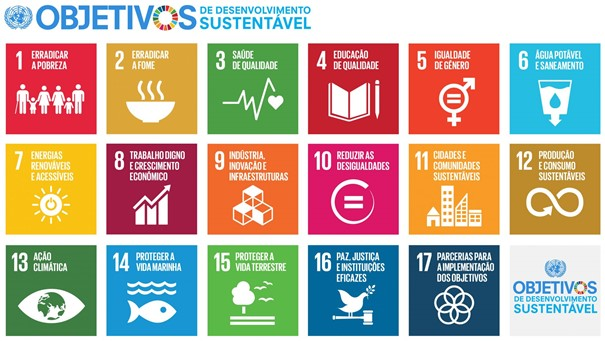
\includegraphics{Imagens/DesenvolvimentoSustentavel.jpg}
    \caption{Objectivos de Desenvolvimento Sustentável da ONU}
    \label{fig:ODS}
\end{figure}

\section{Objetivos e Perguntas de Pesquisa\label{se:objetivos}}

Foram aprovadas a nível europeu (2020)\cite{52020DC0299} sugestões de alterações aos serviços de sistema, que serão seguidas pelos Estados-Membros. Nesta dissertação, será realizada a aplicação dessas sugestões, identificando as melhorias em relação ao \textit{design} actual e avaliando se as novas sugestões serão suficientes para garantir a operação de um sistema elétrico \textasciitilde100\% renovável, potencialmente identificando ações adicionais para garantir a robustez e segurança do sistema elétrico sem o uso de combustíveis fósseis.\par
A penetração das \gls{vRES} no sistema de energia eléctrica trouxe maior incerteza na previsão em mercados de energia, pois estas estão mais sujeitos a elementos não controláveis como a velocidade do vento ou a radiação solar incidente.\par
As seguintes perguntas servirão de guia nesta pesquisa:\par

\begin{enumerate}[label=\alph*)]
  \item Podemos reduzir a incerteza na produção criada pela participação das \gls{vRES} nos sistemas de energia? 
  \item A alocação dinâmica pode ter um efeito positivo no mercado de reservas?
  \item É possível prever a necessidade de reserva necessária baixando a alocação desperdiçada?
\end{enumerate}

Para responder às perguntas \textit{supra} referidas, utilizaremos dados de previsão de geração de energia renovável para estimar a energia necessária para alocação secundária. Actualmente, os valores de previsão desse mercado estão distantes do consumo real, o que resulta em alocações no dia anterior que não estão em conformidade com as necessidades reais.\par
O objetivo deste trabalho é criar métodos de previsão para o dia seguinte, da necessidade de alocação de banda de reserva secundária, de modo a alocar banda suficiente e, simultaneamente, baixar a alocação em excesso, usando dados históricos das mesmas.\par
Iremos explorar a optimização da fórmula de alocação de banda de reserva da REN, testando novos valores para o parâmetro horário da mesma.\par
Utilizando técnicas de \textit{machine learning} vamos criar um modelo para a previsão de alocação necessária do dia seguinte.\par
Previsões mais exactas tornam possível uma melhor gestão das alocações, resultando num menor gasto de recursos energéticos e financeiros.\par

\section{Organização do Documento \label{se:organização}}

Este documento está dividido em capítulos. Sendo que os primeiros apresentam uma introdução às ideias e temas no 1, o estado de arte dos temas na literatura publicada, seguido de uma contextualização do tema do trabalho proposto no capítulo 2. Dentro da contextualização é de forma geral apresentado os mercados de energia, os sistemas de reserva, e os métodos de previsão para os mesmos, dentro destes o uso de fórmulas e o uso de \textit{machine learning}, formulando aqui a motivação e caminho de estudo.\par
No capítulo 3 apresentamos no sub-capítulo Ferramentas as bibliotecas criadas em \textit{python} para o presente estudo.
Segue o sub-capítulo Métodos onde abordamos os diferentes estudos presentes, como serão dirigidos e condições a alcançar. Dividindo o trabalho em estudos distintos para o tipo de previsões apresentadas no capítulo 2.
Métricas e Dados intitula o capítulo 4 que começa numa dissecção das métricas aplicadas ao longo das experiências e como estas influenciam a mesma, terminando num estudo geral dos dados utilizados, seus tratamentos e elações iniciais de análise. Apresentado também o que é usado como treino e como validação para as experiências.
No capítulo 5 são apresentados os resultados da experiência completa, incluindo as métricas apresentadas, apresentado gráficos de séries temporais das previsões conseguidas. Dando realce aos melhores modelos e optimizações conseguidos.
Termina com um breve capítulo conclusivo dando um pouco mais de contexto aos resultados, apresentando possíveis caminhos futuros de melhoria dos mesmos e discutindo o impacto de \textit{machine learning} no futuro das energias renováveis e consequentemente nos mercados de reserva.

% Os dois capítulos seguintes apresentam os dois diferentes estudos. No \hyperref[ch:estudo_1]{capítulo 4} é definido e apresentado o resultado do estudo da estimativa do parâmetro $\rho$ da fórmula de estimativa da \gls{REN}.\par
% No \hyperref[ch:estudo_2]{capítulo 5} explora-se o segundo estudo, o dimensionamento dinâmico da alocação necessária. São apresentados os dados utilizados com um estudo preliminar sobre os mesmos, e o tratamento necessário para usar nos modelos.\par
% No \hyperref[ch:ferramentas]{capítulo 6} as ferramentas de programação criadas para realizar a mesma.\par
% Os 3 capítulos seguintes são os descritivos da experiência em si. \hyperref[ch:metricas]{Capítulo 7} são as métricas usadas e criadas para a validação da experiência, \hyperref[ch:metodos]{capítulo 8} é a estrutura e parametrização da mesma, e \hyperref[ch:resultados_discussao]{capítulo 9} apresenta os resultados.\par
% Termina com um \hyperref[ch:conclusao]{capítulo conclusivo} onde são avaliadas as experiências como um todo, e o seu impacto no âmbito dos mercados de reserva.\par
\label{ch:intro}

% Revisão bibliográfica
\newpage
\thispagestyle{plain}
\chapter{Revisão bibliográfica}

A revisão bibliográfica deve recorrer a normas, livros, artigos científicos e, obrigatoriamente, deve indicar a bibliografia consultada de forma correta com recorrência a um reference manager. A maneira mais usual é adotar o sistema numerado por ordem de aparecimento do texto.\\
Isto é um exemplo de uma equação:

\begin{equation}
\label{eq:eq1}
    a = 1
\end{equation}

A tabela deve ter uma legenda por cima da mesma, tal como o exemplo em baixo. Se os valores da tabela não são calculados pelo autor e referem-se a valores de outros autores tem de constar as respetivas referências aos seus trabalhos.

%Tabela construida com https://www.tablesgenerator.com/

%Para ter a citação em formato [1] usem \cite{}
%Para usar citet ou citep teriam de modificar o style do \usepackage[backend=biber, natbib=true, style=numeric, sorting=none ]{biblatex} style de numerico para authoryear


\label{ch:revisao}

% Contextos
\newpage
\thispagestyle{plain}
\chapter{Contextos\label{ch:contextos}}

\section{Mercado de Serviços de Sistema \label{se:servicos_sistema}}
%\cite{Lopes2021}
%\cite{Watson1984}
%\citep{Schweppe1988}

O mercado de serviço de sistema é parte integrante dos mercados de energia e mantêm responsabilidade sobre a segurança do mesmo.\cite{dgegmss} \\
Serve para garantir o equilibrio entre a energia produzido e a consumida. Esta qualidade e segurança é controlada através da frequência e da potência activa, controlo de tensão e potência reactiva, arranque automático e outras técnicas de sistemas \cite{Rassid2017} \cite{Carneiro2016}. \\
Neste caso de estudo estamos interessados nos serviçoes de controlo de frequência. A nível europeu estes serviços são impostos pela ENTO-E (\textit{European Network of Transmission System Operators for Electricity}), e a operação dos mesmos é da responsabilidade dos TSO (\textit{Transmission System Operator} ou \textit{ Operador da Rede de Transporte}) nacionais.\\
Para manter o controlo de frequência o gestor de sistema deverá manter reservas para responder às diferenças entre a energia consumida e produzida na rede, que deve ser mantida em equilibrio. Quando o serviço de sistema precisa de actuar para manter a frequência no seu valor nominal, 50Hz na Europa, isto é feito alterando a potência activa dos geradores.  \\
Quando é necessário um aumento na potência chama-se a isto Banda de Reserva/Regulação a Subir, e quando é necessária uma diminuição chama-se à mesma a Descer. \\
Para isto, mo mercado ibérico, a tarefa é dividida em três reservas, primária, secundária e terciária. Esta divisão assenta no tempo de resposta que os sistemas precisam de ter, e na capacidade de actuação (MWh/Hz). \\

A reserva secundária, como sistema de segurança à reserva primária, regula-se pelo mercado de banda das reservas secundárias, que decorre no dia anterior ao que será necessário utilização da mesma. \\
Este valor alocado tem um custo para as operadoras, como tal a previsão do mesmo é importante para a gestão destes sistemas de segurança. Estas previsões são feitas através de estatiscas dos sistemas, e tendo em conta as areas de balanço que o mesmo têm. \\
Uma melhor previsão deste valor poderia levar a uma poupança, tanto financeira, como de recursos. \\

Estas previsões são feitas ao uso de formulas. Que por si só não preveêm a variabilidade dos sistemas de produção de energia renovável. Esta variabilidade sendo dificilmente previsivel, tem sido alvo de estudo com modelos de \textit{machine learning} \cite{} \\
Com bons resultados apresentados em estudo de energias renováveis, a aplicação dos mesmos metódos para as reservas de sistema parece um passo natural. \\



%\section{MIBEL \label{se:mibel}}
%\cite{Bessa2012}
%\cite{Carneiro2016}
%\cite{Fernandes2016}
%\citep{Agostini2021}

\label{ch:contexto}
% Dados

\newpage
\thispagestyle{plain}
\chapter{Estudo 1: Estimativa do parâmetro $\rho$ da fórmula da REN}



Para responder a primeira questão estudou-se o comportamento do parâmetro p na equação publicada pela REN para a Banda de Regulação Secundária a Subir:

\begin{equation} \label{eq:BRREN} 
    BR = \rho \times \sqrt{a \times  L_{max} + b^{2}} - b 
\end{equation}
onde:
\begin{itemize}
  \item $BR$: Banda de Reserva  de regulação secundária necessária (MW).
  \item $\rho$: Paramêtro horário.
  \item $a$ e $b$: Coeficientes empiricos, $a$=10MW e $b$=150MW .
  \item $L_{max}$: Pico máximo de consumo (MW).
\end{itemize}

Aqui queremos descobrir qual o valor do parâmetro $\rho$ (por hora do dia) que melhor nos descreve os dados reais. Para isso estudamos os valores reais usados para a Banda de Reserva, os valores resultantes da proposta de $\rho$  em \cite{Carneiro2016} e os valores resultados do estudo aqui proposto. Aproximar o parâmetro $\rho$  utilizando os dados históricos. \\
Todos os dados necessários são disponibilizados pelo operador do sistema no \href{https://mercado.ren.pt/PT/Electr}{site da REN}, com exceção do consumo máximo expectável. Este parâmetro é então substituído pelo consumo real, como uma aproximação à formulação indicada previamente.\\
Os dados estudados contêm entradas horárias desde 2010 até ao fim de 2018. Com as seguintes variáveis:\\

\begin{table}[H] \centering \caption{Dados REN} \begin{tabular}{ll}
\toprule
Variável & Unidades \\
\midrule
BANDA SUBIR & MW \\
BANDA DESCER & MW \\
Consumo real & MW \\
Consumo Máximo ENTSO-E & MW \\
\bottomrule
\end{tabular}
 \end{table}

Na equação \ref{eq:BRREN} BR equivale à soma de BANDA SUBIR e BANDA DESCER, onde aqui é sempre considerado que Banda a subir são $\frac{2}{3}$ da Banda de Reserva total e a Banda a descer é o restante $\frac{1}{3}$. \\
Aqui iremos aplicar o mapa de parâmetro $\rho$ apresentado em \cite{Carneiro2016} na formula \ref{eq:BRREN} para o cálculo da Banda de Reserva Carneiro2016 como benchmark. \\

\begin{table}[H] \centering \caption{Valores de $\rho$ apresentado em \cite{Carneiro2016}} \begin{tabular}{ll}
\toprule
Hora & $\rho$ \\
\midrule
1/2/8/9/24 & 1,6 \\
3/7/10/11/19/20 & 1,4 \\
4 & 1,3 \\
5/6/12/13/14/15/16/17/18/21/22/23 & 1,2 \\
\bottomrule
\end{tabular}
 \end{table}


Por outro lado, usando os dados de consumo real, calculamos o $\rho$ ideal para cada entrada, de onde estudamos a melhor normalização dos mesmos para cada hora. \\
O cálculo deste $\rho_{proposto}$ é apenas a utilização da fórmula \ref{eq:BRREN} mas em função de $\rho$ : \\

\begin{equation} \label{eq:rhoproposed} 
    \rho  = \frac{(BR + b)}{\sqrt{a \times L_max + b^{2}}}
\end{equation}


Arredondando o $\rho_{proposto}$ a uma casa decimal, podemos verificar que o histograma das diferentes propostas difere bastante. Sendo que esta apresenta uma curva de distribuição normal. \\


\begin{figure}[H]
    \centering
    \includegraphics[width=\textwidth]{plots/Histograma_parametro_p.png}
    \caption{Histograma $\rho$}
  \end{figure}


Olhando as distribuições por hora: \\

\begin{figure}[H]
    \centering
    \includegraphics[width=\textwidth]{plots/Valor_do_parametro_p_hora.png}
    \caption{Valor do paramêtro $\rho$ (hora)}
  \end{figure}

O $\rho_{proposto}$ apresenta um grande variabilidade em todas as horas, embora de notar que em todas tem um maior peso perto da mediana. O $\rho$ de comparação embora sempre dentro da distribuição note-se que cai quase sempre em zonas com pouco peso nestes dados históricos. \\
Calculamos $\rho$ possiveis para proposta final usando as seguintes aproximações: média, mediana, e média ponderada ao consumo, e à banda. \\

As distribuições por hora são as seguintes:

\begin{figure}[H]
    \centering
    \includegraphics[width=\textwidth]{plots/Comparação_de_p_propostos_por_hora.png}
    \caption{Histograma $\rho$}
\end{figure}

Todas seguem um percurso semelhante ao longo do dia, o qual também pode ser extrapolado para Carneiro2016. A média e mediana destacam-se seguindo muito parecidas, enquanto que as ponderadas também parecidas entre elas são bastante mais discretas. \\
Para a escolha da normalização deste parâmetro à Hora, estudou-se o erro entre a Banda Reserva calculada através das normalizações e a Banda Reserva disponível nos dados. \\


\begin{figure}[H]
    \centering
    \includegraphics[width=\textwidth]{plots/Comparação_das_metricas_de_Erro.png}
    \caption{Histograma $\rho$}
\end{figure}


\begin{table}[H]
    \caption{Erros de Banda de Reserva por método de normalização $rho$}    
    \resizebox{\linewidth}{!}{\begin{tabular}{lrrrr}
\toprule
 & MAE (MW) & RMSE (MW) & MedianAE (MW) & MAPE (\%)\\
Normalização &  &  &  &  \\
\midrule
Carneiro2016 & 53.07 & 66.54 & 44.53 & 18.70 \\
média & 30.94 & 39.19 & 25.38 & 11.58 \\
mediana & 30.85 & 39.20 & 25.17 & 11.51 \\
média ponderada banda & 32.15 & 40.61 & 26.45 & 12.19 \\
média ponderada consumo & 31.54 & 39.91 & 26.20 & 11.73 \\
\bottomrule
\end{tabular}
}
    \end{table}


A normalização com erros mais baixos é a mediana. Com um erro médio (de todo o histórico) para o consumo real de 11.51\% o que comparando com o benchmark de 18.70\% é uma melhoria  bastante considerável. \\
Comparando as bandas calculadas a uma média em cada hora: \\


\begin{figure}[H]
    \centering
    \includegraphics[width=\textwidth]{plots/média_historica_de_banda_de_reserva.png}
    \caption{Média historica de Banda de Reserva}
\end{figure}

Podemos ver que em termos de média horária, a Banda de Reserva calculada através do $\rho_{proposto}$ apresenta quase uma sobreposição por inteiro ao valor médio real. \\

Retiramos as médias dos erros percentuais e podemos observar: \\

\begin{figure}[H]
    \centering
    \includegraphics[width=\textwidth]{plots/erro_médio_por_hora_banda_de_reserva.png}
    \caption{Erro médio por hora Banda de Reserva}
\end{figure}

Em termos de média diária o erro pelo método proposto está bem abaixo da margem de erro do 5\% na banda, em todas as horas. E na outra tese apenas 10\% cai dentro dessa margem de erro. \\

Como tal o $\rho_{proposto}$ a partir do estudo dos dados  históricos é: \

\begin{table}[H] \centering \caption{Valores de $\rho$ propostos} \begin{tabular}{rr}
\toprule
Hora & $\rho$ \\
\midrule
1 & 1.621694 \\
2 & 1.576623 \\
3 & 1.486929 \\
4 & 1.364176 \\
5 & 1.313958 \\
6 & 1.318832 \\
7 & 1.504499 \\
8 & 1.612361 \\
9 & 1.638188 \\
10 & 1.613728 \\
11 & 1.601277 \\
12 & 1.485861 \\
13 & 1.451995 \\
14 & 1.457233 \\
15 & 1.440454 \\
16 & 1.421988 \\
17 & 1.424636 \\
18 & 1.420682 \\
19 & 1.553086 \\
20 & 1.588201 \\
21 & 1.480219 \\
22 & 1.478815 \\
23 & 1.474412 \\
24 & 1.635658 \\
\bottomrule
\end{tabular}
 \end{table}


% \begin{table}[H]
%     \caption{Valores de $\rho$ propostos}    
%     \resizebox{\linewidth}{!}{\begin{tabular}{rr}
\toprule
Hora & $\rho$ \\
\midrule
1 & 1.621694 \\
2 & 1.576623 \\
3 & 1.486929 \\
4 & 1.364176 \\
5 & 1.313958 \\
6 & 1.318832 \\
7 & 1.504499 \\
8 & 1.612361 \\
9 & 1.638188 \\
10 & 1.613728 \\
11 & 1.601277 \\
12 & 1.485861 \\
13 & 1.451995 \\
14 & 1.457233 \\
15 & 1.440454 \\
16 & 1.421988 \\
17 & 1.424636 \\
18 & 1.420682 \\
19 & 1.553086 \\
20 & 1.588201 \\
21 & 1.480219 \\
22 & 1.478815 \\
23 & 1.474412 \\
24 & 1.635658 \\
\bottomrule
\end{tabular}
}
%     \end{table}

Em relação a perdas por arredondamento, apresento o resultado dos erros por arrendamento em cada um da casas possíveis, concluindo que até à primeira casa decimal, pode ser feito arredondamento do parâmetro $\rho$, sem influenciar muito o erro: \\


\begin{figure}[H]
    \centering
    \includegraphics[width=\textwidth]{plots/Erro_médio_por_hora_Banda_de_Reserva_Arredondamento.png}
    \caption{Erro médio por hora Banda de Reserva (Arredondamento)}
\end{figure}



Neste estudo podemos comprovar que usando um $\rho$ extrapolado dos dados históricos, e um $L_{max}$ sendo o consumo real e não o consumo máximo calculado, os erros médios por hora ficam abaixo dos 5\%.\\ \label{ch:estudo_1}

\newpage
\thispagestyle{plain}
\chapter{Estudo 2: Dimensionamento dinâmico da potência alocada na reserva secundária}

\section{Dados Utilizados\label{se:dadosestudo}}

Os dados em estudo são do mercado energético espanol, retirados do site da \href{https://www.esios.ree.es/es}{ESIOS}.

\resizebox{\linewidth}{!}{\csvautotabular{tabelas/indicators_metadata.csv}}



\subsection{Aquisição dos Dados}

No ambito da automatização destes dados foi modificado o repositorio \href{https://github.com/SanPen/ESIOS}{ESIOS} para ser usado como uma biblioteca de python, aberta, em pypi.\\
Sendo uma ferramenta mais facilmente acessivel para a extrair dados do mercado espanhol, \href{https://pypi.org/project/pyesios/}{pyesios}. \\
No âmbito de automatizar o processo, foram feitas contribuições a esta ferramenta para tornar mais acessível, e uma ferramenta aberta de python\\


\thispagestyle{plain}

\section{Estudo dos dados}

Os dados que proponho a prever são os de Energia Usada na Banda de Reserva Secundária, tanto a subir como a descer: "UpwardUsedSecondaryReserveEnergy","DownwardUsedSecondaryReserveEnergy".\\



\begin{figure}[H]
  \centering
  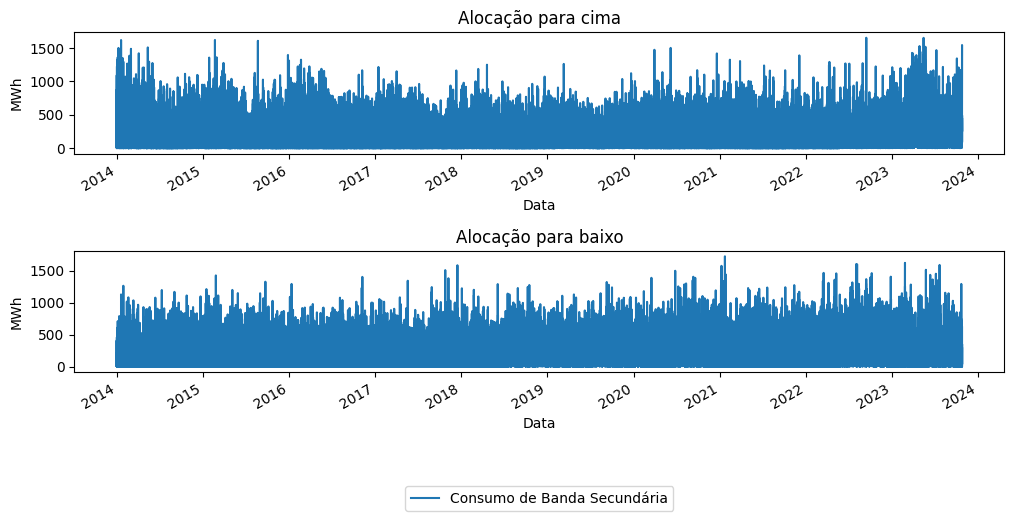
\includegraphics[width=\textwidth]{plots/consumo_originais.png}
  \caption{Serie Temporal dos dados alvo}
  \label{fig:targettimeseries}
\end{figure}


Para termos uma melhor percepção dos mesmos segue algumas janelas temporais mais pequenas.

\begin{figure}[H]
  \centering
  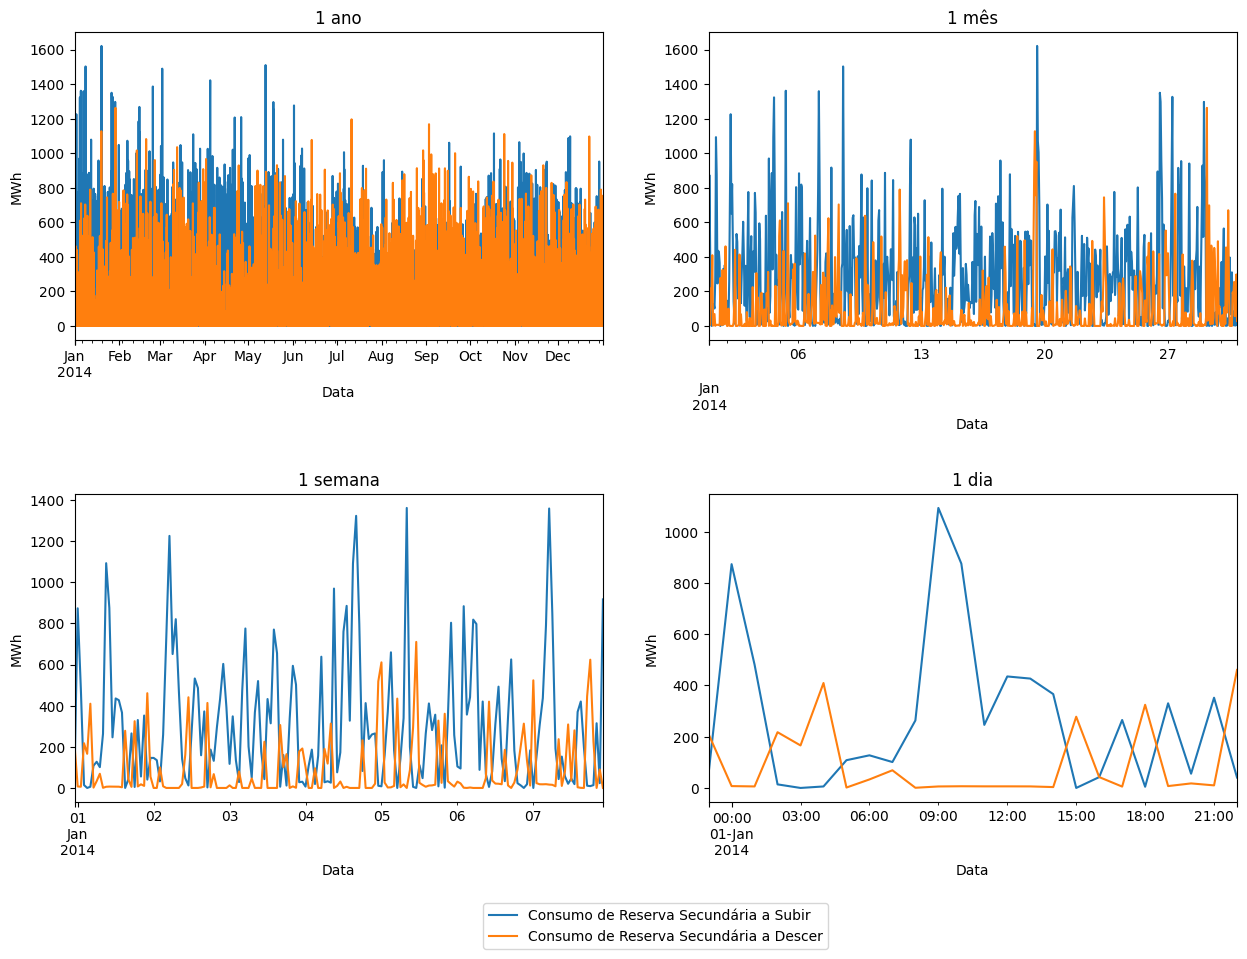
\includegraphics[width=\textwidth]{plots/target_timeseries_windows.png}
  \caption{Janelas Temporais dos dados alvo}
  \label{fig:targettimeserieswindows}
\end{figure}


Estas mostram claramente que ambos os atributos mantêm um comportamento tanto discreto, como linear, isto é, que ou existe algum valor, ou é zero, e se existe valor este tem comportamento linear.\\
A distribuição destes dados é claramente exponencial. O que é importante para a escolha de alguns parâmetros na modelação. \\

		
\begin{figure}[H]
  \centering
  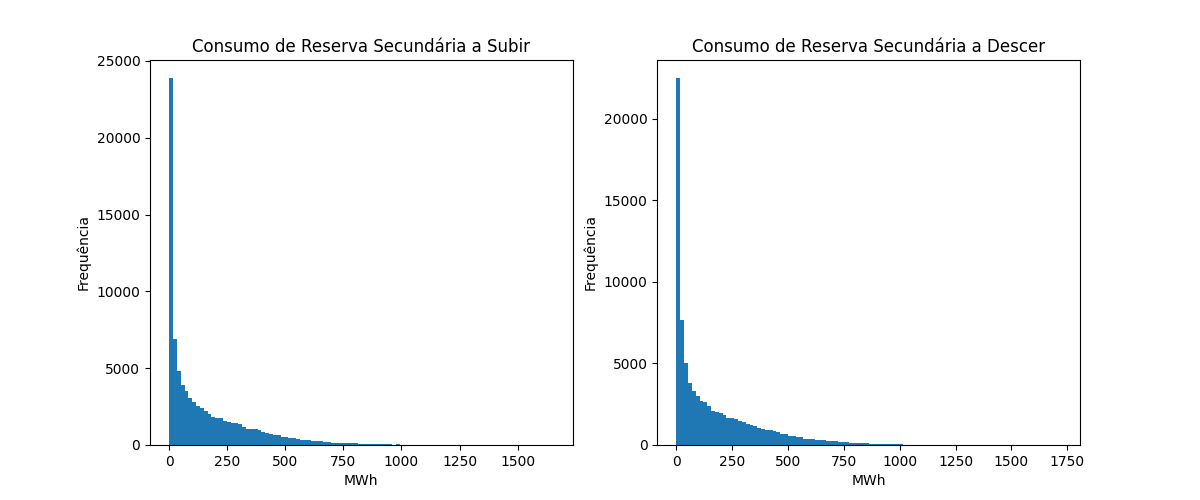
\includegraphics[width=\textwidth]{plots/target_histograms.png}
  \caption{Frequência dos dados alvos}
  \label{fig:targethistograms}
\end{figure}


\subsection{Correlações}

Os modelos vão depender bastante de correlação entre variáveis.

Nesta secção queremos tentar identificar se há visiveis relações entre as variáveis, e se há relações temporais  visiveis nas colunas alvo.


\subsubsection{Correlações entre atributos}


\begin{figure}[H]
  \centering
  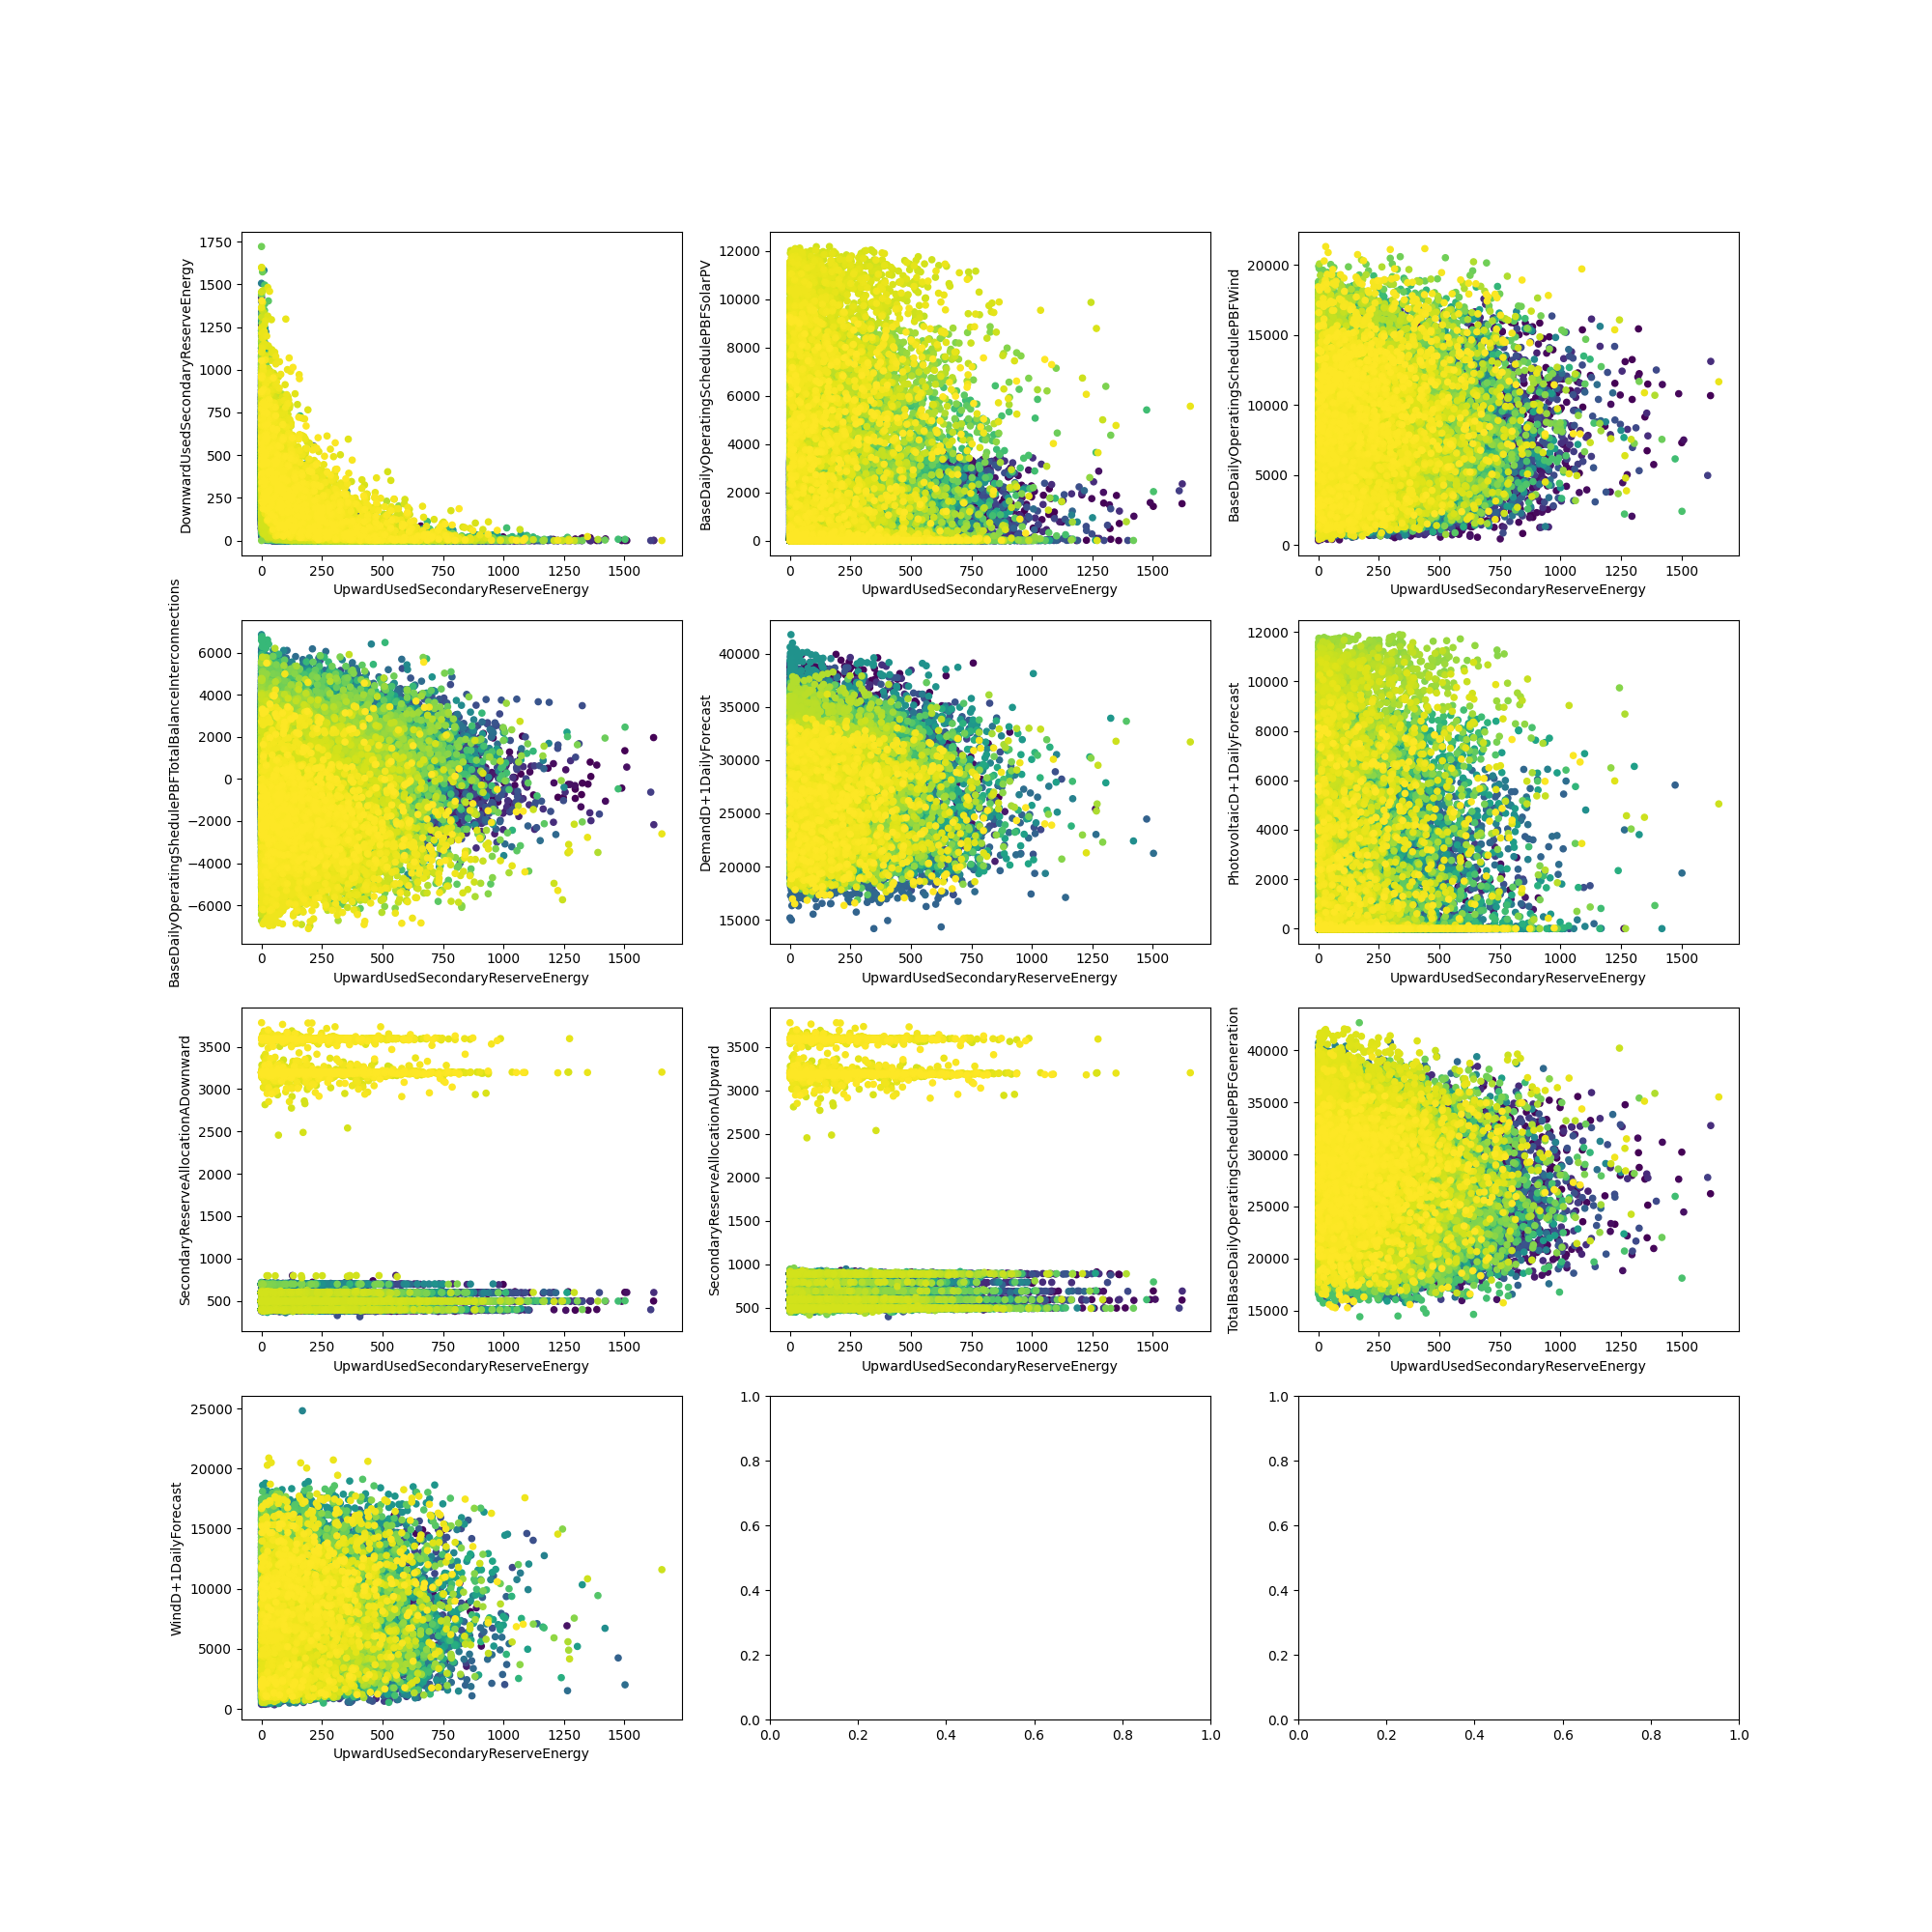
\includegraphics[width=\textwidth]{plots/feature_correlation.png}
  \caption{Correlação entre atributos}
  \label{fig:featurecorrelation}
\end{figure}

Esta figura apresenta a dispersão de valores entre a energia usada, primeiras três linhas a energia para cima e as seguintes a energia para baixo, e os outros atributos presentes.\\
As correlações entre variáveis parecem muitos escassas, o que apresenta já que a previsão destes dados usando estas variáveis vai ser um problema difícil.\\
Por norma é feito uma seleção de atributos baseado nestas correlações, eliminando assim os atributos que ajudam menos, ou até prejudicam os modelos.\\
Segue os valores de correlação onde podemos ver numericamente que existe muito pouca correlação entre os atributos. Onde a primeira coluna são os valores de correlação para a energia usada a subir e a segunda coluna as correlações da energia usada a descer.\\

\begin{figure}[H]
  \centering
  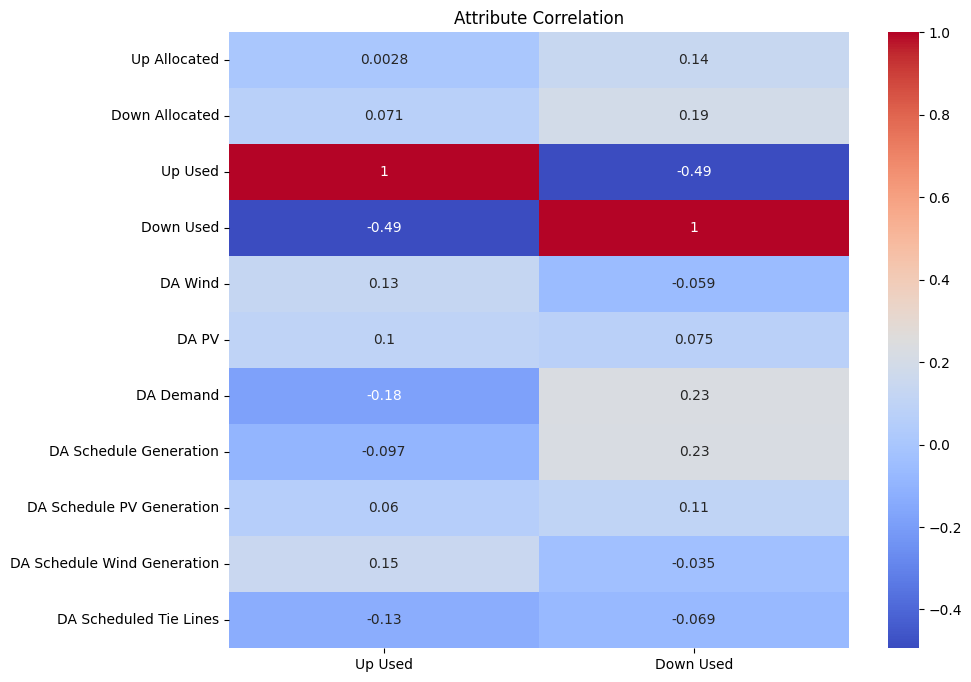
\includegraphics[width=\textwidth]{plots/correlation_heatmap.png}
  \caption{Valores de correlação entre atributos}
  \label{fig:correlationheatmap}
\end{figure}

\subsubsection{Correlações Temporais}

\begin{figure}[H]
  \centering
  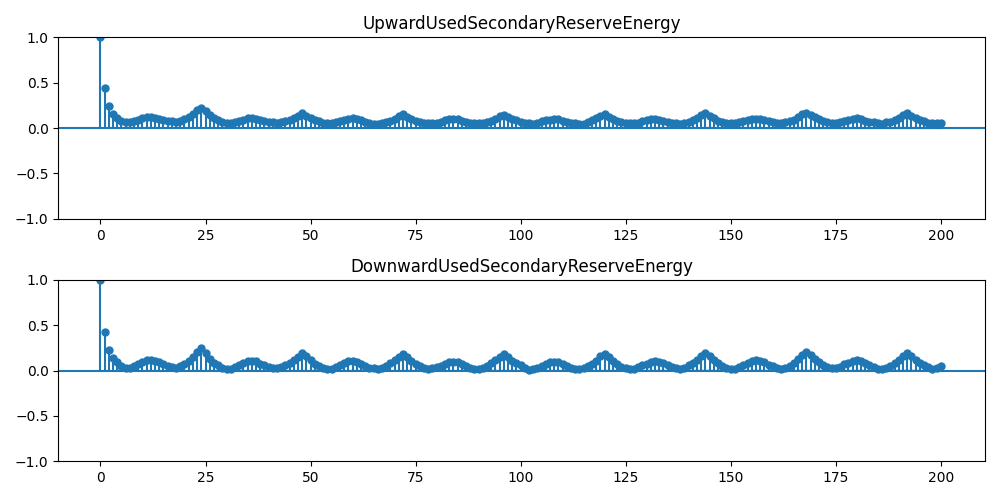
\includegraphics[width=\textwidth]{plots/autocorrelation.png}
  \caption{Autocorrelação Temporal}
  \label{fig:autocorrelation}
\end{figure}

A autocorrelação, em ambos os alvos, é mais forte nas 3 horas mais próximas, e nos pontos com diferença de 12 e 24 horas. \\
É de notar que estes valores são baixos, prometendo já também uma baixa regressividade temporal. \\
Os melhores saltos temporais e suas correlações são mostradas na tabelas em baixo:\\


\begin{table}[H]
  \caption{Autocorrelação Temporal}    
  \resizebox{\linewidth}{!}{\begin{tabular}{lllllllllll}
\toprule
\midrule
\multirow[t]{2}{*}{UpwardUsedSecondaryReserveEnergy} & horas & 1 & 2 & 24 & 23 & 25 & 168 & 144 & 192 & 48 \\
 & rácio & 0.44 & 0.24 & 0.22 & 0.19 & 0.19 & 0.17 & 0.16 & 0.16 & 0.16 \\
\cline{1-11}
\multirow[t]{2}{*}{DownwardUsedSecondaryReserveEnergy} & horas & 1 & 2 & 24 & 23 & 25 & 168 & 144 & 192 & 48 \\
 & rácio & 0.43 & 0.22 & 0.25 & 0.20 & 0.19 & 0.21 & 0.19 & 0.20 & 0.19 \\
\cline{1-11}
\bottomrule
\end{tabular}
}
  \label{tab:tempcorr}
  \end{table}

Outro ponto a denotar é que os objectos não têm um comportamento completamente linear, i.e., parece existir um comportamento discreto na questão ser alocado ou não esta reservas secundárias, e caso seja alocado, aí existir alguma linearidade. \\
Logo qualquer tipo de modelação terá de resolver primeiramente este problema. \\
Estas relações mostram que em termos de atributos usados vai ser um desafio complicado para qualquer tipo de modelo. \\
No âmbito desta dissertação queremos verificar a qualidade das previsões usando estes mesmo atributos, logo, não será feita seleção dos mesmos. \\
A nível da relação temporal, a maior parte dos modelos que iremos testar aplica um janela na dimensão temporal, usando todos os valores nessa janela, e aplicando os pesos nessas distâncias que mais se enquadram. Logo também não é relevante escolher apenas as distâncias temporais com maior correlação, pois os modelos vão fazer essa pesagem. \\


 \label{se:dadoscrus}



\thispagestyle{plain}



\section{Tratamento dos dados}

\textbf{Normalização} \\
A normalização foi deixada por ser aprendida nos modelos, sendo que todos têm como segunda camada, uma de normalização. \\

\textbf{Limpeza} \\

Podemos ver pelos gráficos seguintes que a existem alguns outliers, sendo estes definidos como 3 desvios padrão de distância à média. \\
Estes gráficos mostram também que existe uma variação do que são os valores normais de cada atributo a nível temporal. Logo um método de limpeza não se poderia basear apenas numa definição geral de outliers, mas teria de ser feito em janelas temporais. \\
Pelo mesmo argumento e visto que os outliers fazem parte do que queremos também descobrir, não é aplicada nenhum método de remoção dos mesmo, sendo os dados passados a cru para os modelos. \\


\begin{figure}[H]
  \centering
  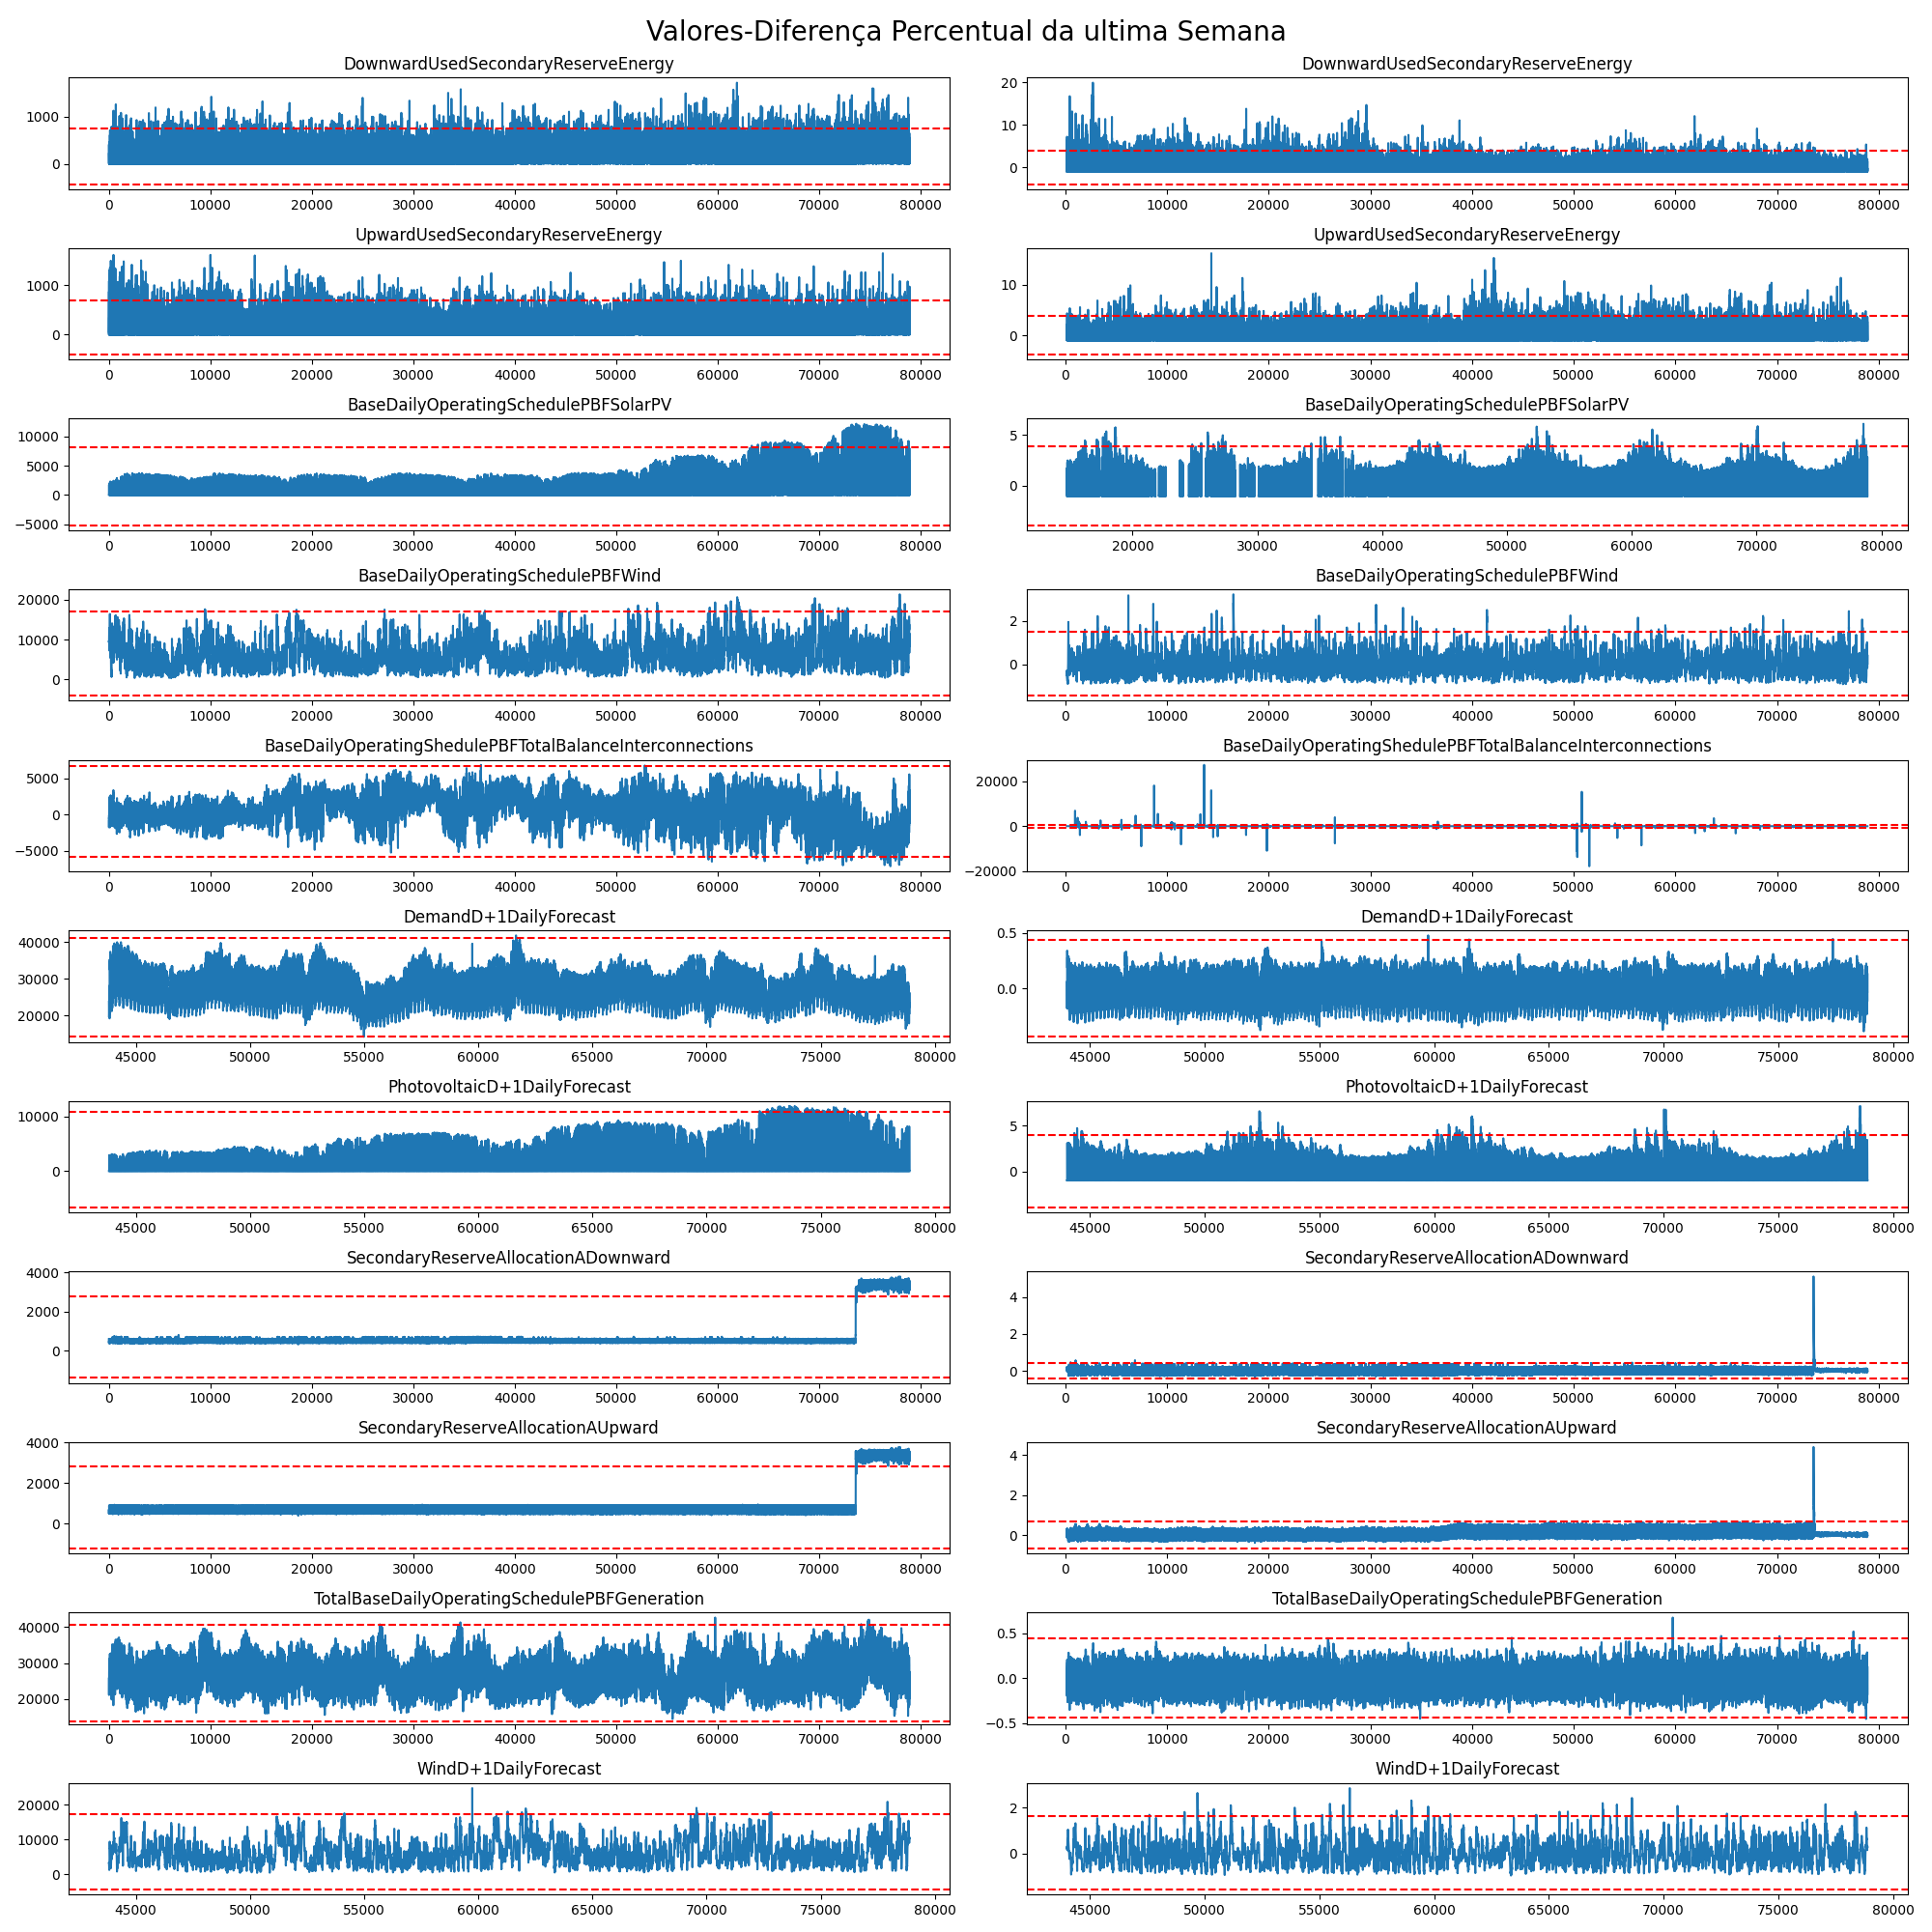
\includegraphics[width=\textwidth]{plots/Outliers_3stds.png}
  \caption{Outliers}
\end{figure}

Outra análise desta variação dos atributos a nível temporal leva-nos a que qualquer divisão dos dados para treino e teste deva levar as variações em consideração. Isto sendo que o treino deve ter representatividade de todas, ou maior parte, das condições diferentes. \\


\textbf{Dados em falta (Missing Data)}

Estudemos também o caso de dados em falta. Alguns destes atributos têm certas entradas vazias, e como podemos ver alguns não têm alguns anos inteiros.\\
Como queremos usar o máximo de dados possíveis iremos usar técnicas de imputing nesses dados. \\
Podemos ver que temos dados em falta de vários anos, em três atributos, e um tem algumas horas esporádicas em falta nos primeiros anos.\\

\begin{figure}[H]
  \centering
  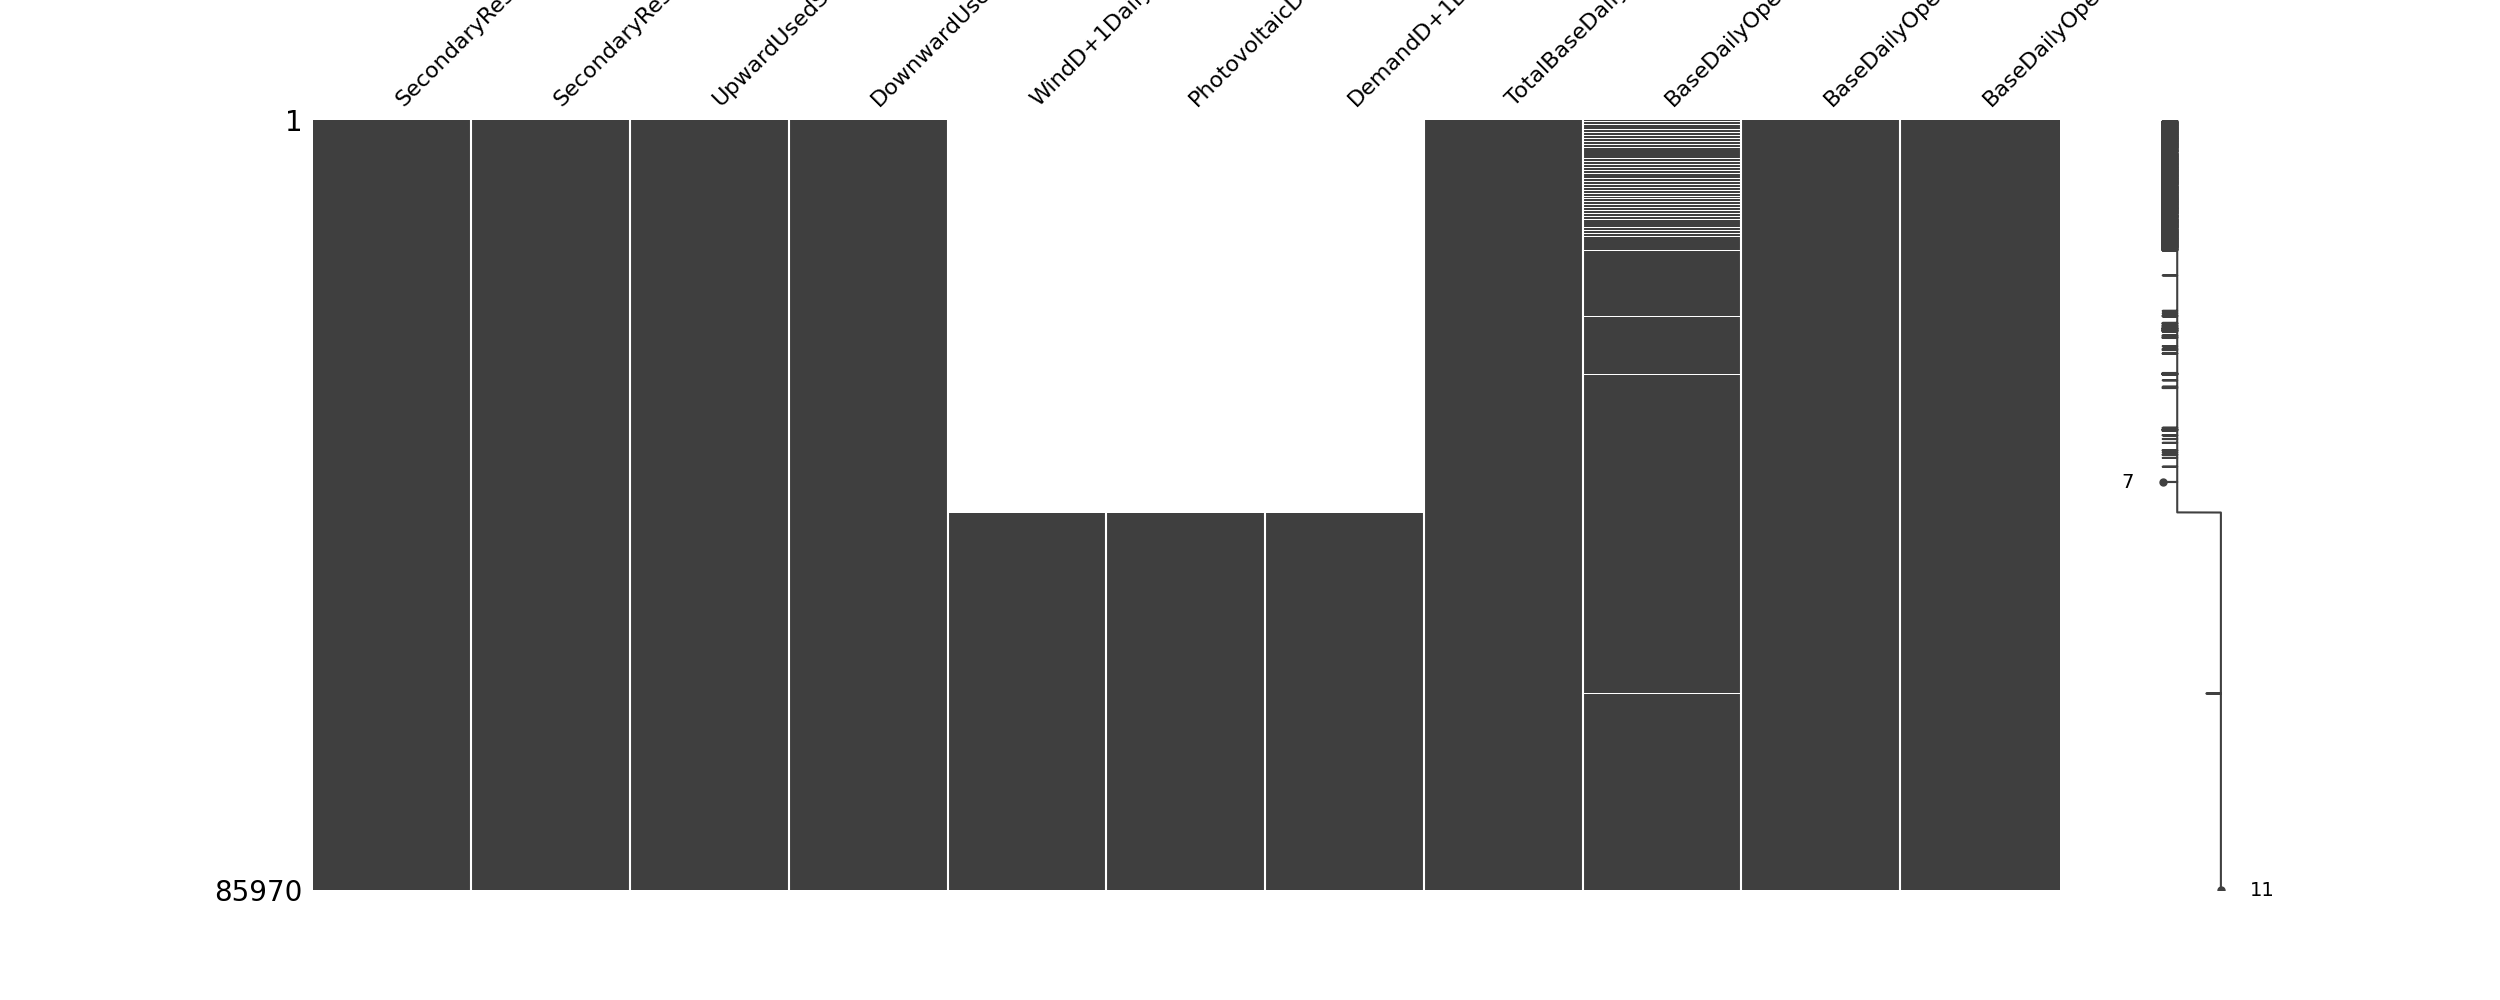
\includegraphics[width=\textwidth]{plots/missing_data.png}
  \caption{Dados em falta}
\end{figure}

Vamos aplicar o método experimental \href{https://scikit-learn.org/stable/modules/generated/sklearn.impute.IterativeImputer.html}{IterativeImputer} da biblioteca de python \href{https://scikit-learn.org/stable/index.html}{sklearn}. \\
Este metodo é baseado nos trabalhos de \cite{vanBuuren2011} e de \cite{Buck1960}

Por ultimo foi adicionado ao dados mais atributos, sendo eles todos de cariz temporal. É adicionado atributos correspondentes à hora, ao dia do ano, ao dia da semana, ao dia do mês, mês, ano. \\

 \label{se:tratamentodados}

\subsection{Dados de treino}

Após o tratamento apresentado as estatísticas gerais dos dados usados para treinar o modelo são:

\begin{table}[H]
    \caption{Dados de Treino}    
    \resizebox{\linewidth}{!}{\begin{table}[H] 
    \caption{Training data summary. \label{training_data_sum}}
    \newcolumntype{C}{>{\centering\arraybackslash}X}
    \begin{tabularx}{\textwidth}{CCCCC}
    \toprule
    & \textbf{mean}	& \textbf{std}	& \textbf{min} & \textbf{max}\\
    \midrule
    Down Used & 168.20 & 199.67 & 0.00 & 1721.40 \\
    Up Allocated & 662.94 & 150.62 & 399.00 & 958.00 \\
    Down Allocated & 549.27 & 126.67 & 312.00 & 956.00 \\
    Up Used & 158.10 & 191.62 & 0.00 & 1654.80 \\
    DA Wind & 5824.12 & 3413.15 & 71.33 & 20879.30 \\
    DA PV & 1666.31 & 2719.60 & 0.00 & 14925.30 \\
    DA Demand & 27944.24 & 4479.39 & 14170.00 & 41773.00 \\
    DA Schedule Generation & 27249.43 & 4603.58 & 13470.50 & 42707.60 \\
    DA Schedule PV Generation & 1714.09 & 2815.35 & 0.00 & 16358.90 \\
    DA Schedule Wind Generation & 6525.51 & 3582.36 & 308.60 & 21619.60 \\
    DA Scheduled Tie Lines & 290.58 & 2157.11 & -7817.00 & 6858.50 \\
    \bottomrule
    \end{tabularx}
    % \noindent{\footnotesize{\textsuperscript{1} Tables may have a footer.}}
\end{table}

}
    \end{table}
 \label{ch:estudo_2}


% Arquiteturas a estudar
\newpage
\thispagestyle{plain}
\chapter{Arquitecturas de Modelos\label{ch:arquiteturas_modelos}}

Grande parte da literatura sobre previsões em modelos de apredizagem apresenta as mesmas arquiteturas, sendo que são depois aprimoradas consoate os dados e o problema. \\
Apresento aqui as aquiteturas mais usadas em previsões, como tambem algumas usadas noutros ramos tentado prever a compatibilidade neste problema. \\
As arquitecturas irão seguir um esquema logíco comum, um bloco de camadas de entrada, um bloco principal e um por fim um bloco interpretativo. \\
As dimensionalidades destas camadas é o que irá formar as diferentes arquitecturas em estudo. \\

\section{Camadas\label{se:layers}}

Para uma construção de modelos usando a ferramenta \href{https://keras.io/}{keras} a unidade básica são as camadas. Estas representação um operação, com uma entrada, e uma saida, e com possiveis parametrizaçoes específicas. \\
Estas camadas ligadas entre si, perfazem um \"profundo\" de camadas neuronais, chamado profundo pois tem mais  que uma camada. \\

Apresento aqui as camadas utilizadas nos modelos aplicados.

\subsection{Dense\label{se:dense_layer}}

A camada dense pega num input, 

\subsection{Convolution\label{se:conv_layer}}
\subsection{MaxPooling\label{se:max_pooling}}
\subsection{\href{https://keras.io/api/layers/regularization_layers/dropout/}{Dropout}\label{se:dropount}}

Dropout é uma camada que elimina/ignora alguns dos neuronios da camada anterior. Este procedimente impede o overfitting, ajudando na generalização. \\
(ref) na imagem
\begin{figure}[H]
	\centering
	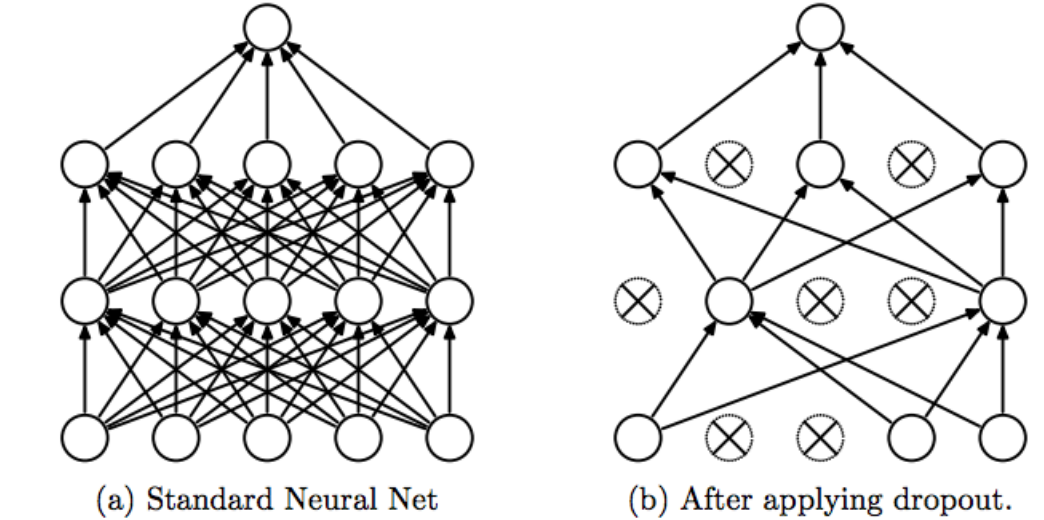
\includegraphics{Imagens/dropout.png}
	\caption{Ilustrção do efeito da camada de dropout}
	\label{fig:dropout}
\end{figure}



\section{Blocos\label{se:blocos}}

Todas as arquiteturas em análise irão ter por base um bloco de camadas neuronais. A formação dessas arquitecturas passa pelas diferentes maneiras que se pode utilizar o bloco principal. Repetições em serie ou em paralelo são um exemplo. \\

\subsection{Bloco Dense\label{se:dense}}

O bloco dense sendo ele o mais simples é formado por duas camadas Dense \cite{}, em que a primeira apresenta um numero maior de filtros que a segunda. \\
Estas camadas não são mais do que uma criação de filtros aleatórios combinando as entradas, para criar todos os filtros de saida. São a base das camadas intrepretativas. A acumulação em série (stacked) de camadas de dense está ligada a melhorias nas capacidades predictivas dos modelos \cite{VLHelen2021}. \\
Exemplo ilustrativo do nosso bloco basico onde entrariam 16 filtros na primeira camada e para finalizar o bloco com 2 filtros \\

\begin{figure}[H]
	\centering
	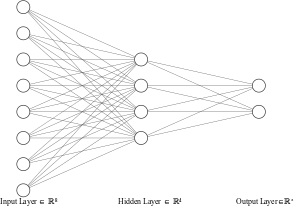
\includegraphics{Imagens/dense_layer.png}
	\caption{Bloco Dense}
	\label{fig:dense_blcok}
\end{figure}
	
\subsection{Blcoo CNN\label{se:cnn}}

Bloco de CNN é aqui definido como uma convolução na dimensão temporal seguido de camadas para combater o overfitting, MaxPooling e Dropout. \\
Normalmente usada em processamentos de imagens, o uso de convuluções temporais é tambem por si mesmo uma ideia forte. \\

explicar om que e CNN
imagem

Usada tambem as ideias de attention, residual e o que eu chamei broad


\subsection{Blcoo LSTM\label{se:lstm}}

O uso de LSTM para previsões é uma area comum, mas aqui é seguido através das ideas partilhas em \cite{Hewamalage2021}, e reforçado pelo uso em previsões energéticas demonstados em \cite{Costa2022} \\
O bloco LSTM é a aplicaçao das RNN, aqui sendo apenas definido como uma camada de LSTM. \\
Estes blocos mantêm dentro de si ligações a diferentes camadas temporais, e cada filtro criado, mantêm uma "memória" dos filtros passados. \\
Bastante utilizado em modelação de linguagem.

imagem


\section{Arquiteturas \label{se:arquitecturas}}

\subsection{Vanilla \label{se:vannila}}

O termo "Vanilla" aqui é aplicado para aquitecturas que apenas usam um bloco de cada, um de entrada, um principal, e um interpretativo. \\
Como exemplo a arquitetura de "VanillaCNN"

imagem da mesma

\subsection{Stacked\label{se:stacked}}

Stacked refere-se a "amontoado" onde se utiliza o bloco principal várias vezes em série.E apenas um bloco de  entrada e um interpretativo. \\
Como exemplo a arquitetura de "StackedCNN"

imagem da mesma

\subsection{MultiHead\label{se:multihea}}

Multihead é o termo para quando os blocos de entrada e principais são repetidos paralelamente, um caminho para cada atributo, ou uma outra paralelização à escolha. Sendo depois concatenadas essas camadas e passadas juntas para a camada interpretativa. \\
Aqui foi usado sempre a paralelização por atributos, e ao invês de fazer Mulithead no sentido de multiplas entradas, para simplicidade de programação, foi feito um paralização interna no modelo, apos a camada de entrada, onde a mesma é repetida para cada atributo. \\
Foi testado a diferença, e para os dados usados não havia diferenças de qualidade, mas sim em tempo de treino, logo a mais rapida foi a escolhida. \\
Como exemplo a arquitetura de "MultiheadCNN"

imagem da mesma

\subsection{MultiTail\label{se:multitail}}

Esta arquitectura tem o mesmo conceito que a anterior a nivel de paralelização, mas neste caso esta é feita apenas na camada interpretativa. Sendo que o resultado do bloco principal é repetido para criar a paralelização. \\
Neste caso foi paralelizado com o numero de tempos a prever, 24 horas, 24 objectos de saida destas modelos.  \\
A grande diferença desta arquitectura para a "Vanilla" que preve 24 horas, é que aqui cada hora tem o seu proprio valor de função de perda, logo o modelo como que está a treinar 24 modelos diferentes, e no caso "Vanilla" a função de perda é ùnica e é a media do erro das horas todas. \\
Como exemplo a arquitetura de "MultiTailCNN"

imagem da mesma

\subsection{UNET\label{se:UNET}}

Normalmente usando em modelção de imagens, a arquitectura UNET passa por criar uma rede de expansão dos filtros, usando convoluções, e de seguida uma rede de contracção dos mesmo, até aos tamanhos pretendidos.\\
O bloco principal contextualmente o mesmo que o CNN.\\
Nas suas ligações UNET junta informação de filtros passados (não de nivel temporal mas de rede neuronal) para realçar informação já trabalhada, e assim identificar padrões de vários contextos diferentes.\\
É habitual tambem adicionar aos blocos principais portões de atenção, portões residuais. Estas duas tecnicas são tambem estudadas aqui.\\
É chamada assim pois é uma rede (NET) que forma um U na sua expansão e contracção.\\

Como exemplo a arquitetura de "UNET"

imagem da mesma


\section{Considerações adicionais\label{se:modelos_plus}}

Aqui e dizer que os modelos utilizados para teste sao as combinacoes deste blocos nestas aquiteturas.

Imagens de layers criadas com 
dense
http://alexlenail.me/NN-SVG/index.html\label{ch:arch}
% Ferramentas
\newpage
\thispagestyle{plain}
\chapter{Ferramentas}

\section{\href{https://github.com/alquimodelia/forecat/tree/main/forecat}{Forecat}\label{se:forecat}}


Com o propósito de desenvolver este estudo, e deixar ferramentas para a replicação do mesmo, foi criado uma biblioteca em python para desenhar as arquitecturas em estudo.\\

\subsection{Construtor de modelos}

Seguindo as arquitecturas descritas anteriormente esta ferramenta constrói os modelos automaticamente, sendo que precisamos apenas de fornecer os parâmetros variáveis.\\
O construtor assenta na ideia de três camadas abstratas de redes neuronais. A camada de entrada, a camada de bloco, e a camada interpretativa.\\
A camada de entrada recebe os dados e normaliza, podendo também fazer outras operações de preparação para a camada de bloco.\\
A camada de bloco é a camada descritiva da arquitetura, é a que tem as operações fundamentais.\\
A camada interpretativa é a que recebe o sinal de múltiplas redes neuronais internas, e traduz para o objectivo, usando Dense layers. \\

Esta abstração segue sempre esta ordem. As variações dentro de cada arquitetura dependem das governamentalizações das mesmas, ou de cada camada, ou então da repetição do circuito, em paralelo ou em série. ou uma combinação destes.\\

\subsection{Gerador de dados}

O gerador construido trata da formatação dos dados para entrada nos modelos. Formatação esse que se baseia nos valores de janelas temporais a usar, e na divisão treino/teste.\\
Esta ferramenta agrega os dados em tensores de formato \textit{(N, t, a)}, onde \textit{N} é o número de casos, \textit{t} é a janela temporal, e \textit{a} é o número de atributos.\\
A ferramenta permite também definir o tempo de salto entre cada entrada.\\
Usando como exemplo uma janela temporal de 168 (horas, uma semana) para treino, e 24 (horas) para o alvo. Com um salto temporal de 1 a primeira entrada teria como treino as primeiras 168 horas dos dados, e como alvo as 24 horas consequentes. A segunda entrada seria a partir da segunda hora dos dados, e assim consecutivamente. Para um caso em que o tempo de salto seria 24, a primeira entrada mantinha-se, mas a segunda começaria 24 horas depois, e não apenas uma.\\

Como estamos também a lidar com dados desfasados, o gerador permite um TODO: shift em atributos a especificar. No caso em estudo temos que os atributos são de DA (day-ahead), logo estão desfasados 24 horas. O que implica termos de aplicar este shift nos dados que não são DA, nomeadamente os dados alvo. Esta propriedade permite também o fácil uso da ferramenta noutros dados desfasados, como as previsões a 3 ou 8 horas.\\

\section{\href{https://github.com/alquimodelia/MuadDib}{MuadDib}\label{se:muaddib}}

Esta ferramenta criada para desenvolver as experiências desta dissertaçao, permite ao utilizador apenas com os dados que quer utilizar e a especificaçao das metricas pretendidas, facilmente ter um modelo optimizado para os seus dados e problema. \\
Criada especificamente no ambito deste trabalho, está focada em criaçao de previsões, podendo no entanto ser utilizada para outros fins. \\
A configuração é bastante facil de usar, e tem em conta um publico não especializado. O que significa que qualquer utilizador com um conjunto de dados pode fazer previsões utilizando machine learning.

\label{ch:ferramentas}
\newpage
\thispagestyle{plain}
\chapter{Métricas}

As métricas utilizadas serviram maioritariamente dois propósitos, com valorizações distintas na escolha de melhores modelos. \\
O primeiro intuito é de estudo de cada modelo, utilizando as métricas comuns de regressão linear, comparando os valores reais com os valores das previsões.\\
Outro objectivo das métricas aplicadas e este mais relevante, era o estudo comparativo do desempenho de cada modelo com o modelo de benchmark.\\


\begin{itemize}
    \item $t$: Valor real.
    \item $p$: Previsão.
    \item $n$: número de amostras.
  \end{itemize}


\section{Métricas de modelo}

\bigskip
RMSE - Root Mean Squared Error \\

\begin{equation} \label{eq:rmse} 
    RMSE = \sqrt{\frac{1}{n} \sum_{i=1}^{n}(t_i - p_i)^2} 
\end{equation}
\smallskip

Métrica comum em problemas de regressão, dando mais peso a erros maiores, mas retorna um valor que pode ser diretamente comparado ao valor em estudo. Neste caso podemos considerar que o RMSE representa o erro quadrático em MWh. \\
\bigskip
SAE - Sum Abs Error \\


\begin{equation} \label{eq:sae} 
    SAE = \sum_{i=1}^{n}\left|t_i - p_i \right|
\end{equation}
\smallskip

Este simboliza a soma absoluta de todos os erros, dentro da janela temporal em questão. Que representa a quantidade total da energia alocada/não alocada em erro, este é também a soma das duas próximas métricas.\\
\bigskip
AllocF - Alocação em Falta \\

\begin{equation} \label{eq:allocf} 
    AllocF = 
    \begin{cases} 
        0 & , \text{se } p \geq t \\
        t - p  & , \text{se } p < t \\
    \end{cases} 
\end{equation}
\smallskip

Representa a soma total de toda a energia que faltou ser alocada. \\
\bigskip
AllocD - Alocação em Demasia \\

\begin{equation} \label{eq:allocd} 
    AllocD = 
    \begin{cases} 
        0 & , \text{se } p \leq t \\
        p - t  & , \text{se } p > t \\
    \end{cases} 
\end{equation}
\smallskip

Representa a soma total de toda a energia que for alocada em demasia. \\

\section{Métricas de comparação modelo/benchmark}

GPD - Ganho Percentual de Desempenho

\begin{equation} \label{eq:gpd} 
    GPD = \frac{SAE_{benchmark} - SAE_{modelo}}{SAE_{benchmark}} \times 100
\end{equation}
\smallskip

O Ganho Percentual de Desempenho é a nossa métrica basilar. Representa, dentro da janela temporal de validação, a percentagem de melhoria do modelo em relação ao benchmark. Isto é representa a percentagem de energia que foi melhor alocada que o modelo. Onde 100\% representa uma melhoria perfeita, onde o modelo não tem erro. E 0\% representa nenhuma melhoria, ou seja, igual ao benchmark. Pode também ter valores negativos, que representa a percentagem em que o modelo é pior que o benchmark, podendo ser infinitamente pior.\\
Esta métrica é representativa da totalidade de energia, tanto alocado como em falta. \\
As próximas métricas são variações desta que ajudam a escolher o melhor modelo em cada experiência, conseguindo distinguir entre alocação em falta e em demasia.\\
\bigskip
GPDF - Ganho Percentual de Desempenho (alocação em) Falta\\

\begin{equation} \label{eq:gpdf} 
    GPDF = \frac{AllocF_{benchmark} - AllocF_{modelo}}{AllocF_{benchmark}} \times 100
\end{equation}
\smallskip

O mesmo que o GPD mas apenas para as somas totais de alocação em falta.\\
\bigskip
GPDD - Ganho Percentual de Desempenho (alocação em) Demasia\\

\begin{equation} \label{eq:gpdd} 
    GPD-D = \frac{AllocD_{benchmark} - AllocD_{modelo}}{AllocD_{benchmark}} \times 100
\end{equation}
\smallskip

O mesmo que o GPD mas apenas para as somas totais de alocação em falta.\\
\bigskip
GPD Norm - Ganho Percentual de Desempenho Normalizado \\

\begin{equation} \label{eq:gpdnorm} 
    GPD Norm = \frac{GPDF + GPDD}{2}
\end{equation}
\smallskip

Aqui o GPD é calculado a partir dos já calculados GPDF e GPDD, sendo a média destes. Desta maneira conseguimos ter uma percentagem de melhoria em relação ao benchmark, onde a melhoria da alocação em demasia e a melhoria da alocação em falta têm o mesmo peso. \\

\bigskip
GPD $Norm^{2}$ - Ganho Percentual de Desempenho Normalizado (negativos) Quadrado

 GPD $Norm^{2}$=GPD norm mas os GPD são ao quadrado se forem negativos  


 \begin{equation} \label{eq:gpdnorm2} 
    GPD Norm^{2} = 
    \begin{cases} 
        GPD Norm & , \text{se } GPDF \text{ }\&\text{ } GPDD \geq 0 \\
        \frac{GPDF^{2} + GPDD}{2} & , \text{se } GPDF  < 0 \\
        \frac{GPDF + GPDD^{2}}{2} & , \text{se } GPDD < 0 \\
    \end{cases} 
\end{equation}
\smallskip


O mesmo que GPD norm mas os GPDF ou GPFD que sejam negativos o seu valor é ao quadrado e mantendo-se negativo. Serve para dar mais peso aos valores negativos, assim não tendo GPD altos mesmo se um dos GPD for negativo (pior que o benchmark). \\
Esta métrica é a principal na escolha do melhor modelo em cada experiência visto manter ambos os GPD mas penalizando se algum deles é negativo. \\
\bigskip
GPD Positivo  - Ganho Percentual de Desempenho Positivo

 \begin{equation} \label{eq:gpdpositivo} 
    GPD Positivo = 
    \begin{cases} 
        GPD & , \text{se } GPDF \text{ }\&\text{ } GPDD \geq 0 \\
        0 & , \text{se } GPDF \text{ }\|\text{ } GPDD < 0 \\
    \end{cases} 
\end{equation}
\smallskip


Esta métrica é igual a GPD mas apenas nos casos em que ambos são positivos, logo o modelo é melhor que o benchmark, senão é zero. Serve para medir o GPD real, mas apenas nos casos em que o modelo já surpassa o benchmark.\\
\label{ch:metricas}

% Métodos
\newpage
\thispagestyle{plain}
\chapter{Métodos}

A todas as experiências foram aplicadas as métricas apresentadas, excepto no benchmark onde teríamos métricas de comparação a ele próprio.\\
Para a escolha de melhor modelo dentro das experiências foi escolhido o modelo que melhor resultados apresentou para a métrica em questão. Sendo esta o GPD $Norm^{2}$ enquanto não encontramos uma melhoria tanto na alocação em falta como na em demasia, ao que se seguida foi usado o GPD Positivo.\\
No caso das Redes Neuronais a hiper parametrização foi feita também deste modo, sendo que primeiro se encontrou uma hiper parametrização adequada aos dados, usando uma arquitetura simples e só depois com essa configuração foi feita a experiência  nas várias arquiteturas.\\
O objectivo é conseguir um modelo que tenha a uma Alocação Total em Falta e Alocação Total em Demasia menor que o Benchmark, dentro dos anos 2019 a 2022. Logo em termos de métricas um GPD Positivo mais elevado possível.\\

\thispagestyle{plain}
\section{Estatisticos}

Em estatística conseguimos encontrar vários métodos de estudo de séries temporais. Estes métodos são normalmente usados como primeira abordagem para fazer previsões.\\
Estes modelos podem ser auto-regressivos (AR), onde vão fazer previsões baseados num número (p) de dados anteriores. Estes modelos são construídos com a noção de que um valor é linearmente dependente de p valores anteriores numa série temporal.\\

\begin{alignat*}{2} 
    & X_{t} : \text{Valor no } t \text{ a prever.} &\quad& p : \text{O número observaçoes anteriores.} \\
    & \varphi_{i} : \text{Coeficiente na observação } i. &\quad& q : \text{O número observaçoes anteriores.} \\
    & \epsilon_{i} : \text{Erro na observação } i. &\quad& \theta_{i} : \text{Coeficiente na observação } i \text{.} \\ 
    & \mu : \text{Média dos valores } X \text{.} 
\end{alignat*}

\bigskip
AR - Auto-Regressivos \\

\begin{equation} \label{eq:ar} 
    X_{t} = \sum_{i=1}^{p}\varphi_{i} X_{t-i} 
\end{equation}
\smallskip

Outra família destes modelos são os de média móvel (MA), onde a média de um número de observações (q) em conjunto com os erros ($\epsilon$) e os coeficientes ($\theta$) é usada para prever os valores seguintes.\\
\bigskip
MA - Média Móvel \\

\begin{equation} \label{eq:ma} 
    X_{t} = \mu + \sum_{i=1}^{q}(\theta_{i} \epsilon_{t-i}) + \epsilon_{t}
\end{equation}
\smallskip
Estes dois tipos de modelos podem ser juntos criando os modelos auto-regressivos de média móvel (ARMA). que junta as capacidades dos modelos anteriores.\\

\bigskip
MA - Média Móvel \\

\begin{equation} \label{eq:ma} 
    X_{t} = \sum_{i=1}^{p}\varphi_{i} X_{t-i}  + \mu + \sum_{i=1}^{q}(\theta_{i} \epsilon_{t-i}) + \epsilon_{t}
\end{equation}
\smallskip

Existem mais modelos de previsão estatística baseados nestes com algumas variações, mas para este trabalho, e apenas como ponto de comparação às redes neuronais, ficamos apenas por estes.\\
As variáveis em estudo por tipo de modelo foram retiradas das autocorrelações temporais usando os métodos de sugestão da ferramenta \hyperref[se:muaddib]{MuadDib}:\\


\begin{table}[h] \centering
\begin{tabular}{lrrrr}
    \toprule
     & p & q \\
    \midrule
    AR & 1/ 2 / 23 / 24 / 25 / 48 / 144 / 168 / 192 / 336 & NA \\
    MA & NA & 1 / 24 \\
    ARMA & 1 & 1 \\
    \bottomrule
    \end{tabular}
    \label{tab:varsstats} 
    \caption{Variáveis de estudo dos modelos AR/MA}
\end{table}


Todos estes modelos foram testados usando o software disponível na package de python \href{https://www.statsmodels.org/stable/index.html}{statsmodel}, com a classe \href{https://www.statsmodels.org/stable/generated/statsmodels.tsa.arima.model.ARIMA.html}{ARIMA}.
 \label{se:metstats}


\newpage
\thispagestyle{plain}
\section{Redes Neuronais}
 \label{se:metneuralnet}

\thispagestyle{plain}
\section{Dados de Validação}
Os dados de validação são os mesmos que os dados de treino, embora apenas durante os anos de 2019 a 2022, inclusive.\\
Usamos como benchmark as capacidades alocadas, "SecondaryReserveAllocationAUpward" e "SecondaryReserveAllocationADownward", e como validação e objectivo, \hyperref[se:metneuralnet]{y}, a própria energia usada, "UpwardUsedSecondaryReserveEnergy" e "DownwardUsedSecondaryReserveEnergy".

\section{Benchmark}

Como método de comparação a todas as experiências foi criado uma base que servirá de benchmark.\\
Este base não é nada mais do que a própria previsão feita pela entidade reguladora ESIOS. Dentro do nossos dados são os valores nos campos "SecondaryReserveAllocationAUpward" e "SecondaryReserveAllocationADownward".\\
Para os dados utilizados, podemos ver a totalidade e comparação do benchmark (Energia Alocada) com a energia utilizada.\\

\begin{figure}[H]
    \centering
    \includegraphics[width=\textwidth]{plots/alocacoes_originais.png}
    \caption{Série Temporal dos dados de Benchmark c/ consumo real}
    \label{fig:benchmarktimeseries}
\end{figure}

Imediatamente podemos verificar que o método para prever a energia necessária actualmente está dentro de um espectro limitado de valores, sendo que esses valores estão perto dos valores de ponta na alocação para cima, e perto dos valores médios na alocação para baixo.\\
Isto deve-se ao facto de ser uma função fixa, baseado no dia em questão. Notamos também que a meio de 2022 houve uma mudança dessa função que limitou os alcances tornando os valores mais elevados. Devido à guerra na Ucrânia e à forte incerteza que esta trouxe aos mercados de eletricidade por causa da crise de gás na Europa, que aumentou significativamente o preço deste recurso e levou à adaptação dos consumidores e países, a Red Eléctrica de España (REE) aumentou as necessidades de reserva secundária para responder a esta incerteza.\\
Do ponto de visto de dados faz sentido para diminuir a quantidade  de vezes em que não é alocada energia suficiente.\\
Mas o mais importante a notar é a forma estática destes métodos, dado a natureza flutuante dos da energia necessária este método apresenta frequentemente um erro grande.\\
Podemos ver em pormenor analisando algumas janelas temporais dentro do período de validação. Vendo o melhor e pior resultado, em termos de erro absoluto, em janelas temporais de ano, mês, semana e dia.\\


\begin{figure}[H]
    \centering
    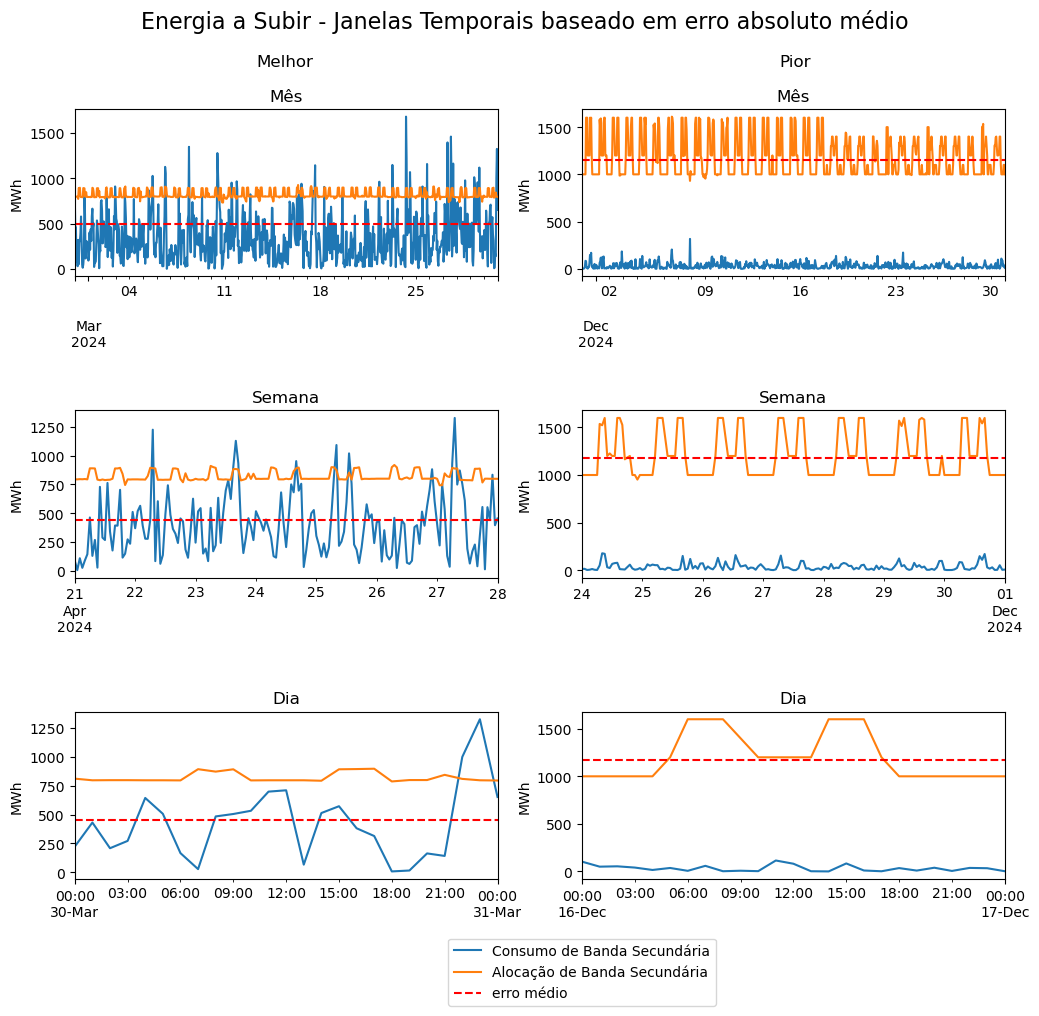
\includegraphics[width=\textwidth]{plots/alocacoes_temporais_upward_dataset.png}
    \caption{Janelas temporais de benchmark energia a subir}
    \label{fig:benchmarktimewindowsup}
\end{figure}


\begin{figure}[H]
    \centering
    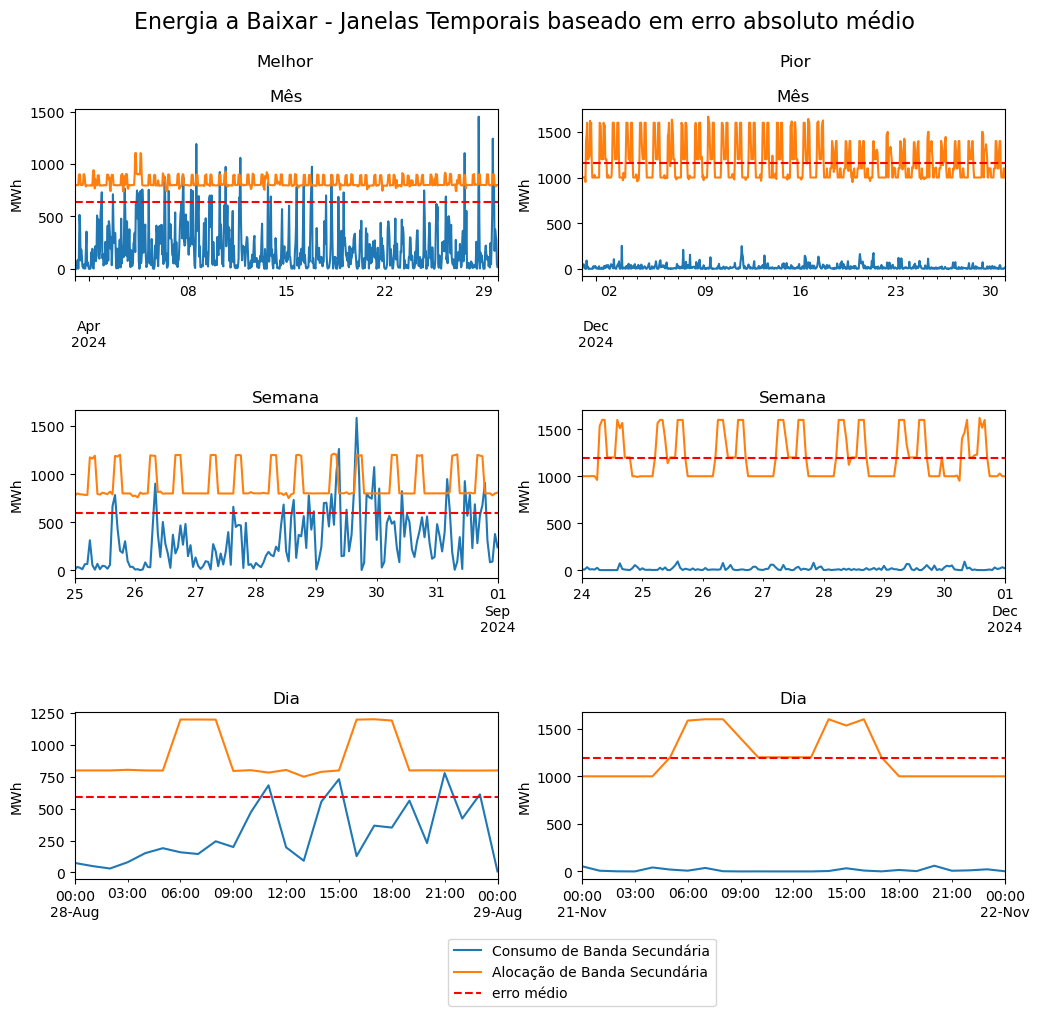
\includegraphics[width=\textwidth]{plots/alocacoes_temporais_downward_dataset.png}
    \caption{Janelas temporais de benchmark energia a descer}
    \label{fig:benchmarktimewindowsdown}
\end{figure}

Dentro destas janelas temporais conseguimos ter melhor a percepção da natureza estática deste modelo actual, e qual longe está dos valores reais necessários.\\





% Neste capitulo percorremos as experiências realizadas. Estas foram feitas atraves do usos do programas criados para o efeito, disponiveis no repositorio GitHub do \href{https://github.com/JotaFan/renewable-generation-into-reserve-markets}{projecto}.\\

% \section{Benchmark}

% Como modelo benchmark iremos usar a alocação feita. Pois são estes valores que procuramos melhorar no caso prático.\\



% \begin{figure}[H]
%     \centering
%     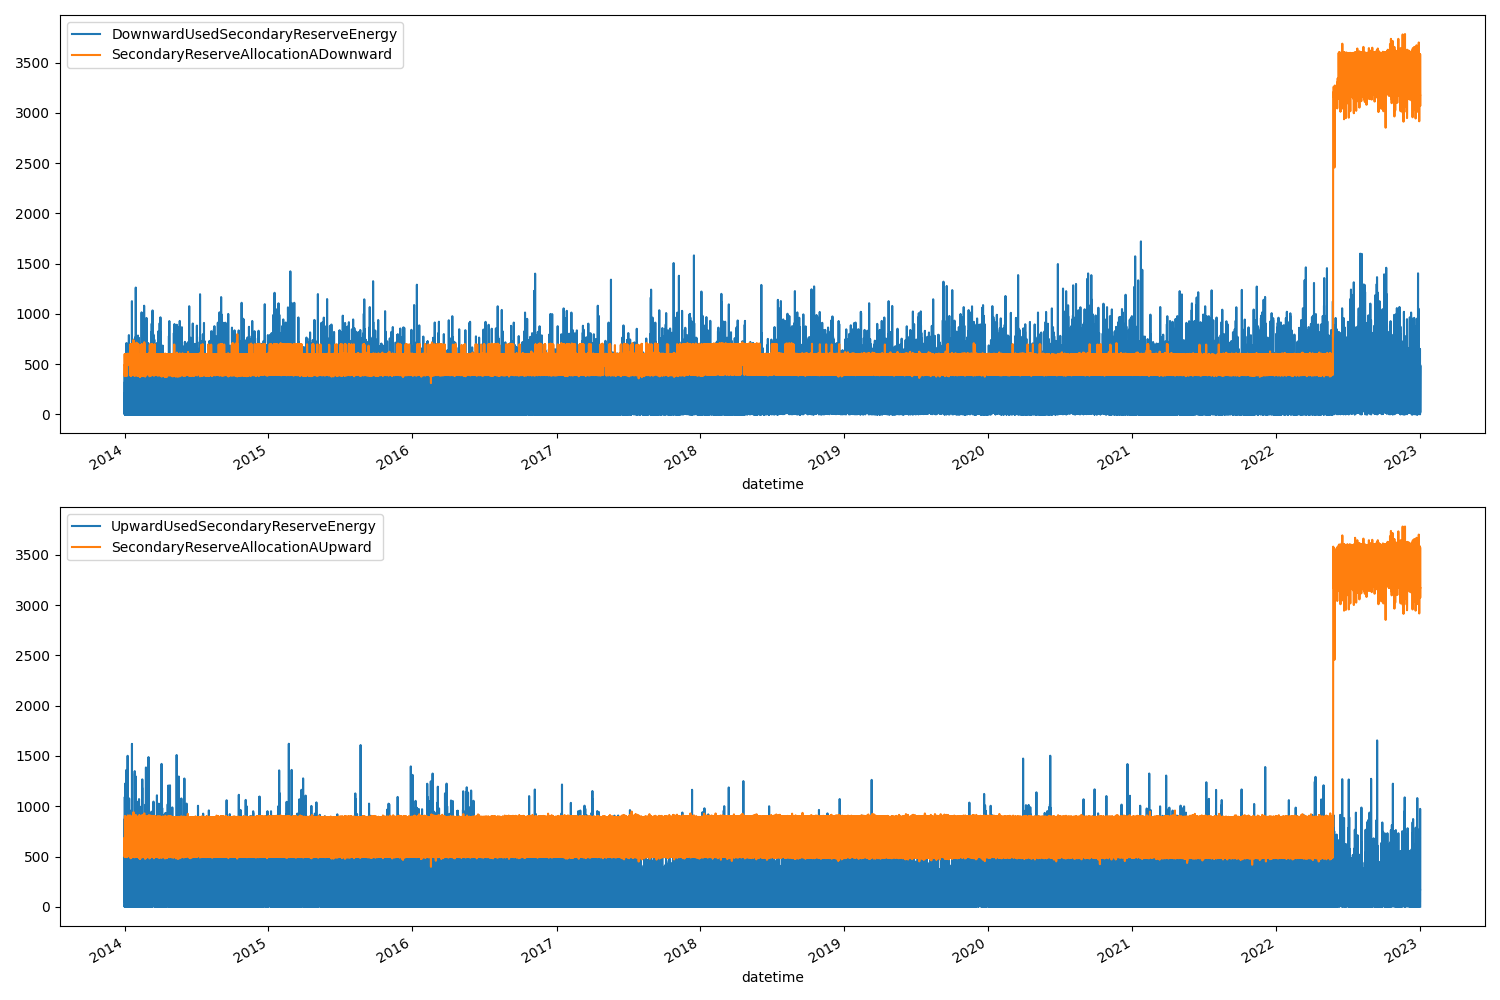
\includegraphics[width=0.8\textwidth]{plots/benchmark.png}
%     \caption{Serie Temporal do benchmark}
%     \label{fig:benchmark}
% \end{figure}
  

% \begin{table}[H]
%     \caption{Dados Benchmark}
%     \resizebox{\linewidth}{!}{\csvautotabular{../data/benchmark_scores.csv}\label{tb:benchmark}}       
% \end{table}


% Para validação dos mesmo, vamos usar o ano 2021, devido aquele salto nos valores de alocação em 2022.\\

% Para esses temos os seguintes dados:

% \begin{figure}[H]
%     \centering
%     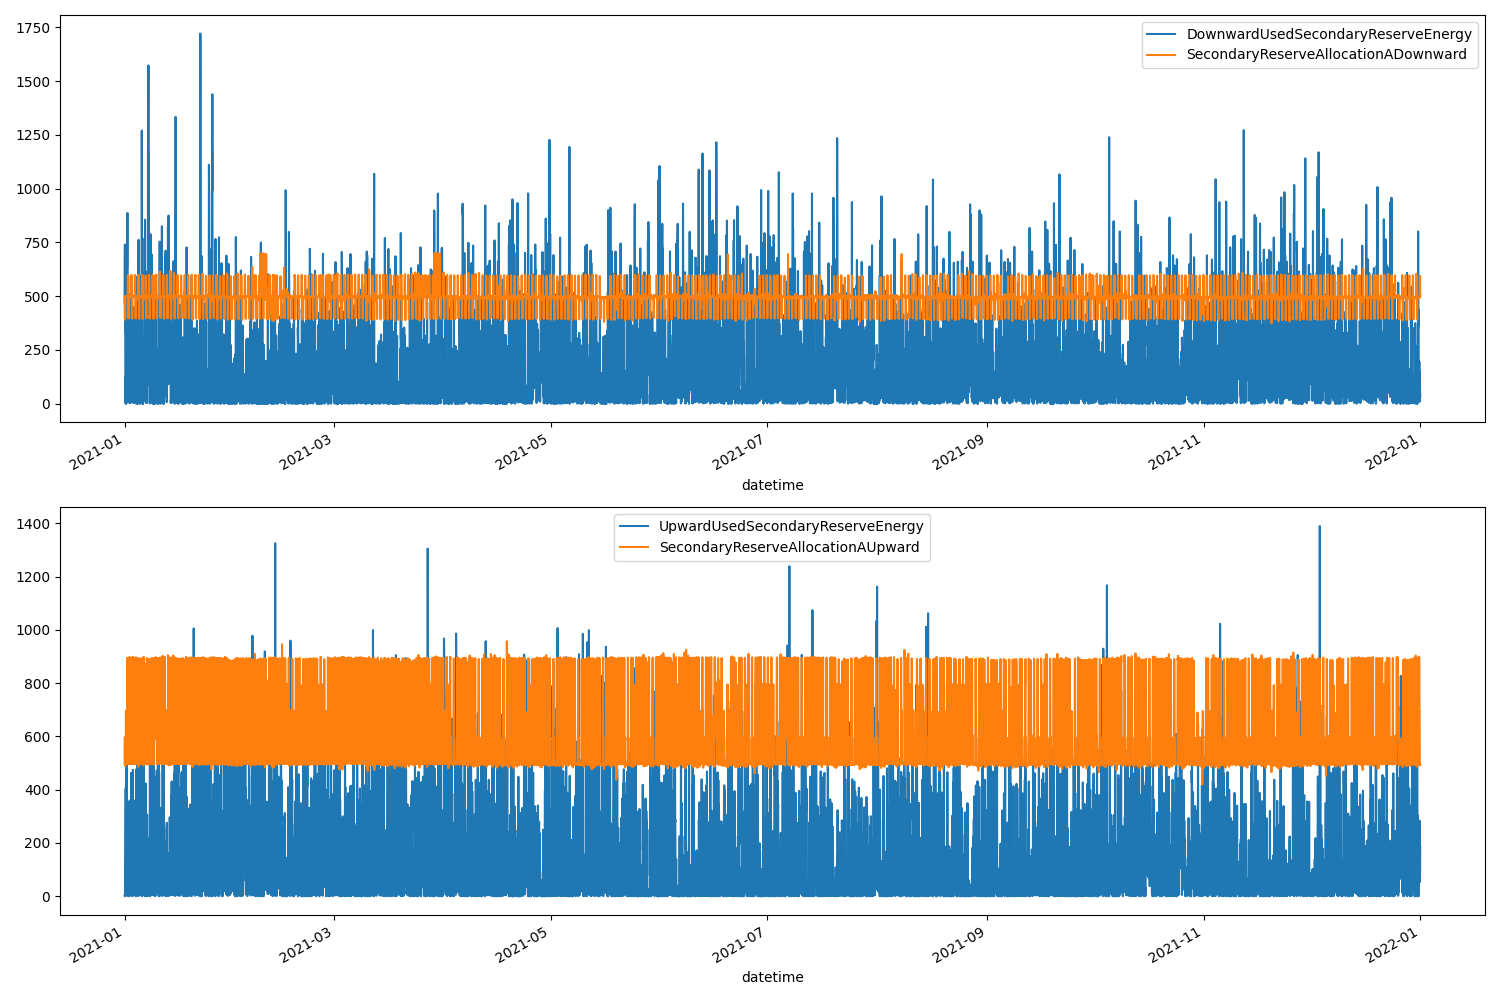
\includegraphics[width=0.8\textwidth]{plots/benchmark_validation.png}
%     \caption{Serie Temporal do benchmark 2021}
%     \label{fig:benchmark_validation}
% \end{figure}
  

% Os metodos em estudo vão ser comparados a esta medida. Sendo que o principal é baixar tanto a alocação perdida, como a alocação a mais. Que se traduzem no erro absoluto.\\

% \begin{table}[H]
%     \caption{Dados Benchmark de validação}
%     \resizebox{\linewidth}{!}{\csvautotabular{../data/benchmark_validation_scores.csv}  \label{tb:benchmark_val}}      
% \end{table}

% \section{Modelos estatiscos\label{se:model_stats}}

% Antes de entrar para o densenvolvimento de modelos vamos usar metódos e modelos abertos para usar comparativamente.\\

% Os modelos estatiscos recurrentes em previsões são AR, MA, ARMA, ARIMA, SARIMA para previsões so com um atributo, e para multiplos atributos VAR.\\
% O modelo AR e o VAR não obtiveram resultados aplicaveis, logo foram desconsiderado.\\

% \subsection{Univariate Analysis}

% Estas análises apenas aplicam uma formula à variavel em questão.

% \subsubsection{AR}
% \begin{equation} \label{eq:AR} 
%     y_t = \beta_0 + \beta_1 y_{t-1} + \dots + \beta_p y_{t-p} + \epsilon_t 
% \end{equation}
% onde:
% \begin{itemize}
%   \item $y_t$: O valor da serie no tempo $t$.
%   \item $p$: O número de atrasos.
%   \item $\epsilon_t$: O barulho no tempo $t$.
%   \item $\beta$: O coeficiente dos valores em atrasdo.
% \end{itemize}

% \subsubsection{MA}
% MA - Moving Average

% A MA 


% \begin{equation} \label{eq:MA} 
%     y_t = c + \epsilon_t + \theta_1 \epsilon_{t-1} + \dots + \theta_q \epsilon_{t-q}
% \end{equation}

% \begin{figure}[H]
%     \centering
%     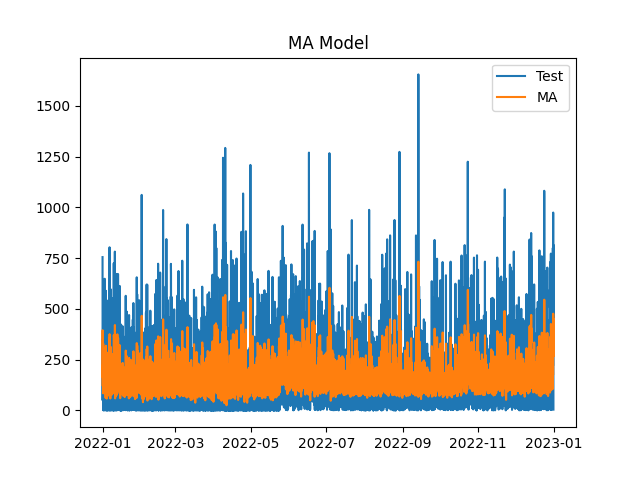
\includegraphics[width=0.8\textwidth]{plots/MA_model.png}
%     \caption{Previsões 2021 com modelo MA}
%     \label{fig:MA_model}
% \end{figure}
  
% \subsection{ARMA}

% AR eé blabla

% \begin{equation} \label{eq:ARMA}  y_t = \beta_0 + \beta_1 y_{t-1} + \dots + \beta_p y_{t-p} + \epsilon_t + \theta_1 \epsilon_{t-1} + \dots + \theta_q \epsilon_{t-q}  \end{equation}
% \textbf{ARMA (Autoregressive Moving Average) Model:}
% \begin{itemize}
%   \item{$y_t$: The value of the time series at time $t$.}
%   \item $p$: The number of time lags to regress on (AR part).
%   \item $q$: The number of time lags of the error term to regress on (MA part).
%   \item $\epsilon_t$: The error term at time $t$.
%   \item $\beta$: The coefficients of the lagged values (AR part).
%   \item $\theta$: The coefficients of the lagged error terms (MA part).
% \end{itemize}


% \begin{figure}[H]
%     \centering
%     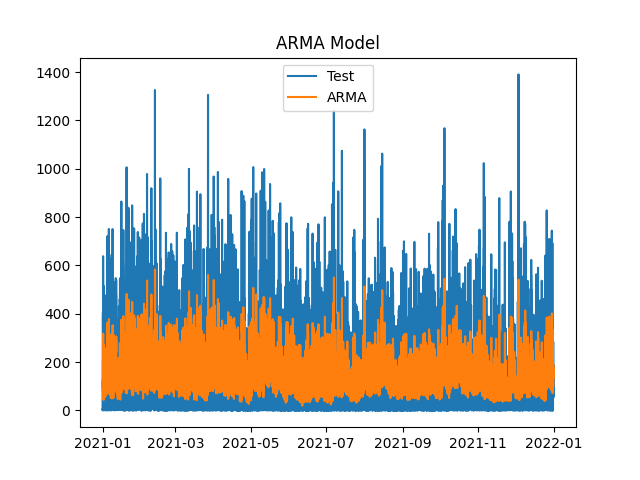
\includegraphics[width=0.8\textwidth]{plots/ARMA_model.png}
%     \caption{Previsões 2021 com modelo ARMA}
%     \label{fig:ARMA_model}
% \end{figure}

% \subsection{ARIMA}

% AR eé blabla

% \begin{equation} \label{eq:ARIMA}y_t^d = \beta_0 + \beta_1 y_{t-1}^d + \dots + \beta_p y_{t-p}^d + \epsilon_t^d + \theta_1 \epsilon_{t-1}^d + \dots + \theta_q \epsilon_{t-q}^d \end{equation}
% \textbf{ARIMA (Autoregressive Integrated Moving Average) Model:}
% \begin{itemize}
%   \item $y_t^{[d]}$: The differenced value of the time series at time $t$.
%   \item $p$: The number of time lags to regress on (AR part).
%   \item $d$: The order of differencing.
%   \item $q$: The number of time lags of the error term to regress on (MA part).
%   \item $\epsilon_t^{[d]}$: The differenced error term at time $t$.
%   \item $\beta$: The coefficients of the lagged values (AR part).
%   \item $\theta$: The coefficients of the lagged error terms (MA part).
% \end{itemize}

% \begin{figure}[H]
%     \centering
%     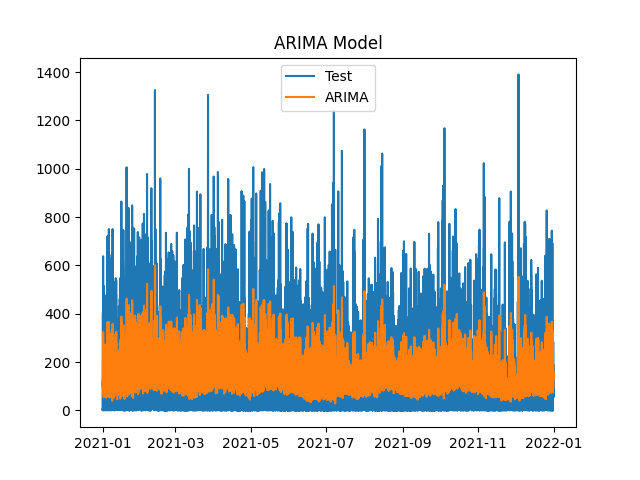
\includegraphics[width=0.8\textwidth]{plots/ARIMA_model.png}
%     \caption{Previsões 2021 com modelo ARIMA}
%     \label{fig:ARIMA_model}
% \end{figure}

% \subsection{SARIMA}

% AR eé blabla



% AR eé blabla

% \begin{equation} \label{eq:SARIMA} y_t^{[m]d} = \beta_0 + \beta_1 y_{t-m}^{[m]d} + \dots + \beta_p y_{t-pm}^{[m]d} + \epsilon_t^{[m]d} + \theta_1 \epsilon_{t-m}^{[m]d} + \dots + \theta_q \epsilon_{t-qm}^{[m]d} \end{equation}

% \textbf{SARIMA (Seasonal Autoregressive Integrated Moving Average) Model:}
% \begin{itemize}
%   \item $y_t^{[m]d}$: The differenced value of the time series at time $t$.
%   \item $p$: The number of time lags to regress on (AR part).
%   \item $d$: The order of differencing.
%   \item $q$: The number of time lags of the error term to regress on (MA part).
%   \item $m$: The number of time lags comprising one full period of seasonality.
%   \item $\epsilon_t^{[m]d}$: The differenced error term at time $t$.
%   \item $\beta$: The coefficients of the lagged values (AR part).
%   \item $\theta$: The coefficients of the lagged error terms (MA part).
% \end{itemize}

% \begin{figure}[H]
%     \centering
%     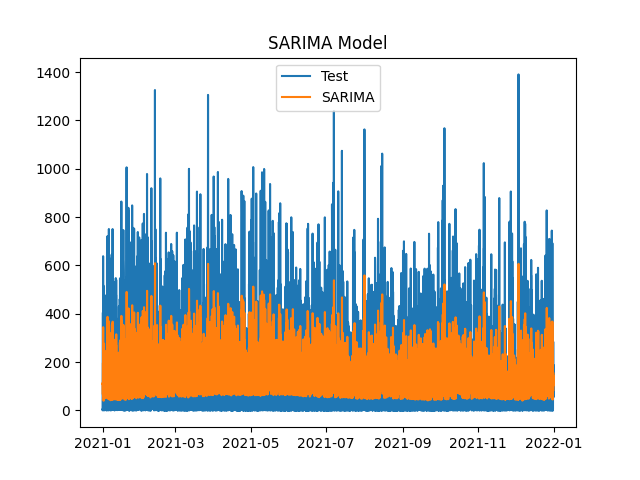
\includegraphics[width=0.8\textwidth]{plots/SARIMA_model.png}
%     \caption{Previsões 2021 com modelo SARIMA}
%     \label{fig:SARIMA_model}
% \end{figure}


% \begin{figure}[H]
%     \centering
%     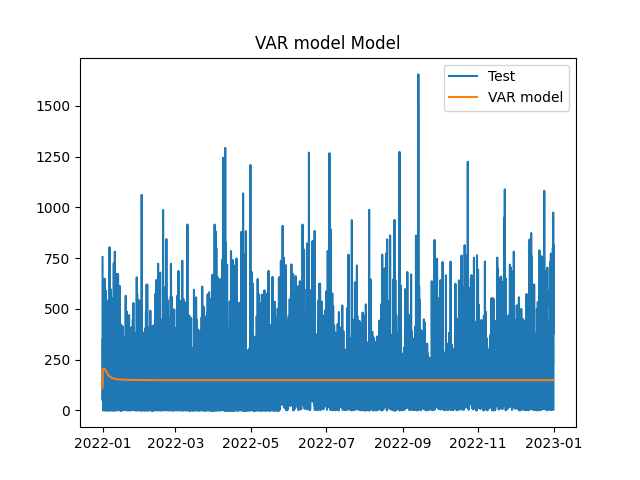
\includegraphics[width=0.8\textwidth]{plots/VAR model_model.png}
%     \caption{Previsões 2021 com modelo VAR}
%     \label{fig:VAR_model}
% \end{figure}









% \subsection{Resultados\label{se:statitics_scores}}

% \begin{table}[H]
%     \caption{Resultados modelos Estatísticos}
%     \resizebox{\linewidth}{!}{\begin{tabular}{llllllllll}
\toprule
rmse & abs erro & erro comp & r2 score & mape score & alloc missing & alloc surplus & optimal percentage & better allocation & beter percentage \\
\midrule
NaN & 0.00 & True & -0.65 & NaN & NaN & NaN & 0.00 & 0.00 & 0.00 \\
171.14 & 1123214.13 & True & 0.14 & 17.04 & 560507.02 & 562707.11 & 63.79 & 63.79 & 86.84 \\
169.99 & 1108555.94 & True & 0.15 & 16.36 & 554443.34 & 554112.60 & 64.04 & 64.04 & 87.17 \\
170.13 & 1111215.12 & True & 0.15 & 16.52 & 556281.62 & 554933.50 & 64.03 & 64.03 & 87.01 \\
171.88 & 1115725.36 & True & 0.13 & 16.43 & 568538.03 & 547187.33 & 63.45 & 63.45 & 86.92 \\
184.60 & 1253196.02 & True & -0.00 & 21.63 & 619929.79 & 633266.23 & 64.82 & 64.82 & 86.07 \\
\bottomrule
\end{tabular}
\label{tb:statitics_scores}}      
% \end{table}

% Apenas pelos métodos estatisticos verificamos que no ano de 2021 teria havido uma melhoria de cerca de 80\% das vezes, usando qualquer um dos métodos apresentados.\\
% Embora a alocação em falta seja de uma ordem de grandeza superior.\\


% \section{Treino e Resultados\label{se:training}}

% Realizaram-se várias experiências, onde em cada um se ia elimando alguns dos objectos em estudo.\\
% Em casa experiências toda a parametrização era igual, à excepção do objecto de estudo.\\

% \subsection{Arquiteturas e numeros de epocas}

% Nesta experiência foi testado o resultado das várias arquiteturas em estudo, como também o impacto do número de epocas na qualidade dos modelos.\\
% As arquitecturas estudadas foram:

% %TODO: arranjar reseach para cada uma 

% \begin{itemize}
%     \item[--] VanillaDense
%     \item[--] VanillaCNN
%     \item[--] VanillaLSTM
%     \item[--] StackedCNN
%     \item[--] StackedLSTM
%     \item[--] EncoderDecoder
%     \item[--] UNET
% \end{itemize}

% O modelos foram treinados em 200 epocas, sendo que foram salvos a cada 10 epocas, de forma conseguirmos perceber os contextos nos saltos de epocas.\\

% As parametrizações usadas:
% \begin{itemize}
%     \item[--] loss : mean squared error
%     \item[--] Metodo activação no meio : relu
%     \item[--] Metodo activação no fim : relu
%     \item[--] optimizador : Adam
%     \item[--] Janela temporal em X : 168 horas (1 semana)
%     \item[--] Janela temporal em Y : 24 horas (1 semana)
%     \item[--] Fracção de treino : 95\%  
% \end{itemize}

% \subsection{Funções de Perda (Loss)}

% TODO: o que é a loss function?

% Esta experiência consiste em rever que função de perda é melhor aplicavel ao problema. Sendo um problema de regressao linear, de valores bastante oscilatórios e com uma distribuição exponencial, temos algumas loss functions que já são reconhecidas para o problema.\\



% \begin{itemize}
%     \item[--] mean absolute error
%     \item[--] mean squared error    
%     \item[--] loss : mean absolute error

% \end{itemize}



% \subsection{Hiperparametrização}

% \subsubsection{Activação}

% \subsubsection{Optimizadores}

% \subsection{Janelas Temporais}

% Um dos pontos deste trabalho é perceber a fesiabilidade de usar dados de previsão do dia anterior (DA) para estes atributos energéticos.\\
% Algo que pode ser também aplicado no futuro a outros dados que não DA, mas sim a 3 horas, ou a 8 horas.\\
% Para perceber esta flexibilidade, mas especialmente para escolher as melhores janelas temporais a usar neste modelos, vamos testar várias combinações.\\
% Mantendo em mente que o objectivo é prever 24 horas, para os casos onde o alvo não dá um previsão de 24 horas, é necessario criar um número de modelos para fazer as 24 horas.\\
% Para validação apenas é usado o espaço temporar previsto, e não multiplos modelos.\\
% Dado as análises de autocorrelação iremos usar como janelas para treino o conjunto [24, 48, 98, 168] para prever o conjunto [1, 4, 8, 12, 24]\\
% Para alem destes foram também testadas combinações com janelas de treino 8 e 12 horas. Estas mostraram rapidamente que janelas de treino menores que as de previsão funcionam muito mal.\\

% \subsection{Classificação}

% Como descrito em (ref)... existe também o uso de tanto classes como valores linears para resolução de problemas de regressão, também chamado \textit{cluster-wise regression}.\\
% Para este teste mudamos um pouco o modelo em uso. Ao invés de apenas uma camada interpretativa, fazemos duas, em paralelo, sendo que uma resolve a regressão e a outra a classificação.\\
% Outro caso, proposto aqui, é usar uma nova camada interpretativa, que combina as duas saidas anteriores (linear e classificação), e resolve novamente para os valores lineares.\\
% Estes modelos não teram apenas uma saida, mas varias, como as arquiteturas MultiTail, mas neste caso cada uma resolve para um problema diferente, com funções de perda, e activações diferentes.\\

% TODO: desenho destas duas camadas intrepretaticas

% \subsection{Pesos}

% Por ultimo foi testado o impacto do uso de pesos nos modelos. Estes pesos são o peso que aquele alvo TODO: epxlicar pesos

% \subsubsection{Modelos lineares}

% Para os modelos lineares o peso que é adiciona ao modelo é a distância à média.\\
% Este peso serve para dar mais importância a valores facilmente considerados outliers.\\



% \subsubsection{Modelos Lineares e de Classificação}
% Aqui o peso é dado por saida. Para as saidas lineares o peso dados é o mesmo que apresentado anteriormente, para a saida de classificação, o peso é o inverso da frequência da classe.\\
% Distribuindo assim a importância de treino pela frquência das classes. Sendo um prática comum especialmente quando as distribuiçoes são muito desiguais, como o caso em estudo.\\
% É aqui estudada a aplicação destes pesos individualmente, e em conjunto. \\
% Os pesos aqui são também normalizados de modo a que o maior peso em cada um deles seja 1, e logo a multiplicação dos dois esteja dentro das mesmas dimensões de relevância.\\


% \begin{equation} \label{eq:peso_media} 
%     P_m = \left| y - mean \right| 
% \end{equation}

% \section{Considerações adicionais  \label{se:metodos_plus}}

% Foram realizados testes adicionais que não obtiveram resultados passivos de boa interpretação, e foram imediatamente descartados, como:

% \begin{itemize}
%     \item[--] Janela temporal em X : 96, 48, 24
%     \item[--] optimizador : todos os optimizadores disponiveis na biblioteca keras
%     \item[--] loss : todas as outra loss functions de regressão disponiveis.
%     \item[--] epocas : influência do número de epocas nos modelos, foram treinados até 20000 epocas alguns modelos mas à medida que a perda ia estagnando na assintomta, o modelo ia apenas piorando.
% \end{itemize}


% Todos os metodos foram realizados utilizando código em python, que está aberto em https://github.com/JotaFan/renewable-generation-into-reserve-markets
\label{ch:metodos}
% Resultados e discussão
\newpage
\thispagestyle{plain}
% \chapter{Resultados e discussão}

% Os resultados das experiências são apresentados por experiência, sendo que cada um vai testando e eliminando parâmetros na modelação.\\
% Após análise inicial na modelação, foi concluído que tentar modelar apenas um dos atributos de cada vez leva a melhores resultados do que tentar modelar os dois no mesmo modelo.\\
% Foi também observado que os dois atributos em questão são análogos, logo os sistemas que melhor representam um dos atributos também são semelhantemente eficazes no outro. \\
% Assim, todas as experiências foram realizadas usando apenas um dos atributos alvo, sendo este o "UpwardUsedSecondaryReserveEnergy", e o atributo de alocação comparativo é "SecondaryReserveAllocationAUpward".\\

% \section{Métricas\label{se:metricas}}

% Para a comparação efetiva dos modelos, iremos usar as seguintes métricas: RMSE, erro absoluto, r2 score, percentagem ótima, alocação em falta, alocação a mais.\\
% As métricas de decisão final são aquelas que representam melhor o objetivo de reduzir os custos de alocação das reservas secundárias, portanto, são as métricas de alocação em falta e em excesso, sendo que a soma delas é o erro absoluto.\\

% \begin{equation}
% \label{eq:rmse}
%     RMSE (y, \hat{y}) = \sqrt{\frac{\sum_{i=0}^{N - 1} (y_i - \hat{y}_i)^2}{N}}
% \end{equation}

% \begin{equation} \label{eq:abse} 
%     \text{Erro Absoluto} = \sum_{i=0}^{N - 1} \left| y_i - \hat{y}_i \right| 
% \end{equation}

% \begin{equation} \label{eq:r2score} R^2\ \text{score} = 1 - \frac{\sum_{i=0}^{N - 1} (y_i - \hat{y}_i)^2}{\sum_{i=0}^{N - 1} (y_i - \bar{y})^2} \end{equation}

% \begin{equation} 
%     \label{eq:miss_alloc} 
%     \text{Alocação em falta} = 
%     \begin{cases} 
%         0 & ,\text{if } \hat{y} \geq y \\
%         y - \hat{y} & ,\text{otherwise} 
%     \end{cases} 
% \end{equation}

% \begin{equation} 
%     \label{eq:opt_perc} 
%     \text{Percentagem ótima} = \frac{1}{N} \sum_{i=1}^{n} 1 [\hat{y}_i \geq y_i  \&  \hat{y}_i \leq \text{alloc}]
% \end{equation}

% Onde $\hat{y}$ são as previsões dos modelos, $y$ são os valores reais utilizados ("UpwardUsedSecondaryReserveEnergy"), e \text{alloc} são os valores alocados ("SecondaryReserveAllocationAUpward"). \\

% \section{Experiências\label{se:experiments}}

% Para a comparação, o erro absoluto para o ano de 2021 na alocação feita é de 3889367.4. \\

% \subsection{Arquiteturas e números de épocas\label{se:archs_epocs}}

% \subsubsection{Arquiteturas\label{se:archs_res}}

% Os três melhores resultados em cada arquiretura com base "alloc missing":

% \begin{table}[H]
% \caption{Resultados Arquiteturas}            
% \resizebox{\linewidth}{!}{\input{../models_validation/linear_models_epocs/experiment_results_best3.tex}}
% \end{table}


% Podemos ver o resultado das metricas principais ao longo das epocas


% \begin{figure}[H]
%     \centering
%     \includegraphics[width=\textwidth]{plots/arch_epocs_results.png}
%     \caption{Resultados arquitecturas/epocas}
%   \end{figure}

% E dado enfase a valores mais perto do benchmark:

% \begin{figure}[H]
%     \centering
%     \includegraphics[width=\textwidth]{plots/arch_epocs_results_near_benchmark.png}
%     \caption{Resultados arquitecturas/epocas}
%   \end{figure}


% Podemos ver que as unicas arquitecturas que atingem valores menores que o benchmark em alloc missing e alloc surplus são UNET e StackedCNN, logo iremos continuar as experiências apenas com essas. \\

% Considerando isso, podemos avaliar apenas tudo o que esteja abaixo do benchmark em alloc missing e alloc surplus.\\

% \begin{table}[H]
%     \caption{Resultados Arquiteturas}            
%     \resizebox{\linewidth}{!}{\input{../models_validation/linear_models_epocs/experiment_results_best_under_benchmark.tex}}
%     \end{table}
    


% \subsubsection{Épocas\label{se:epocas_res}}

% \subsection{Funções de Perda (Loss) \label{se:loss_exp}}


% \begin{table}[H]
% \caption{Resultados Funções de perda}        
% \resizebox{\linewidth}{!}{\begin{tabular}{lrrlrrrrrrr}
\toprule
name & rmse & abs erro & erro comp & r2 score & mape score & alloc missing & alloc surplus & optimal percentage & better allocation & beter percentage \\
\midrule
StackedCNNmsle & 290.70 & 2299543.31 & True & -1.48 & 54.80 & 193283.75 & 2106259.56 & 86.34 & 86.34 & 92.14 \\
UNETmse & 180.84 & 1269085.40 & True & 0.04 & 23.32 & 521000.39 & 748085.00 & 68.78 & 68.78 & 87.31 \\
StackedCNNwl & 175.87 & 1186767.36 & True & 0.09 & 20.02 & 572945.10 & 613822.26 & 64.92 & 64.92 & 86.81 \\
VanillaCNNmse & 162.44 & 1038022.80 & True & 0.23 & 14.30 & 568479.54 & 469543.26 & 61.02 & 61.02 & 87.08 \\
StackedCNNmse & 176.71 & 1103152.68 & True & 0.08 & 14.81 & 673158.53 & 429994.14 & 58.75 & 58.75 & 85.68 \\
StackedCNNmsde & 612.31 & 4978280.05 & False & -10.00 & 81.86 & 3325165.78 & 1653114.27 & 18.27 & 18.06 & 30.14 \\
UNETwl & 30011.42 & 141637978.61 & False & -26431.60 & 2558.08 & 10334.28 & 141627644.33 & 9.35 & 8.62 & 9.91 \\
VanillaCNNwl & 1071.18 & 8912349.22 & False & -32.67 & 171.33 & 63940.63 & 8848408.59 & 1.01 & 0.62 & 3.89 \\
VanillaCNNmsle & 1250.10 & 10759371.90 & False & -44.86 & 201.97 & 0.00 & 10759371.90 & 0.22 & 0.00 & 0.22 \\
UNETmape & 3545800.24 & 18933122401.84 & False & -368973766.69 & 276314.32 & 0.00 & 18933122401.84 & 0.00 & 0.00 & 0.00 \\
\bottomrule
\end{tabular}
}
% \end{table}

% A nivel de percentagem de modelo melhor, elas esão todas bastante renhidas, mas ha uma claro vantagem quando vemos a percentagem de melhor alocação ou de alocação optima.\\
% Sendo que a perda que avança é a de MSLE (Mean Square Log Error).\\
% Esta perda é tendicionalmente usada para distribuições exponencias, e onde temos bastantes outliers, que devem ser considerados. O que é o caso no nosso problema.\\
% Esta experiência valida a observação feito na análise estatistica sobre o mesmo.\\

% \subsection{Hiperparametrização\label{se:hiper}}

% \subsubsection{Activação\label{se:activ}}

% \begin{table}[H]
% \caption{Resultados Ativação}    
% \resizebox{\linewidth}{!}{\begin{tabular}{lrrlrrrrrrr}
\toprule
name & rmse & abs erro & erro comp & r2 score & mape score & alloc missing & alloc surplus & optimal percentage & better allocation & beter percentage \\
\midrule
StackedCNN relu relu & 207.66 & 1113406.16 & True & -0.27 & 3.90 & 1028475.81 & 84930.35 & 38.64 & 38.64 & 82.31 \\
StackedCNN tanh tanh & 236.24 & 1289434.20 & True & -0.64 & 0.85 & 1288660.90 & 773.30 & 11.47 & 11.47 & 80.40 \\
StackedCNN relu tanh & 236.24 & 1289434.20 & True & -0.64 & 0.85 & 1288660.90 & 773.30 & 11.47 & 11.47 & 80.40 \\
StackedCNN relu softsign & 236.31 & 1290138.00 & True & -0.64 & 0.86 & 1289376.80 & 761.20 & 11.29 & 11.29 & 80.40 \\
StackedCNN linear tanh & 236.24 & 1289434.20 & True & -0.64 & 0.85 & 1288660.90 & 773.30 & 11.47 & 11.47 & 80.40 \\
StackedCNN softsign linear & 1112.70 & 8936608.01 & False & -35.34 & 178.94 & 8185.60 & 8928422.41 & 7.99 & 7.50 & 8.60 \\
StackedCNN softsign softsign & 236.24 & 1289436.03 & True & -0.64 & 0.85 & 1288662.99 & 773.04 & 11.00 & 11.00 & 80.39 \\
StackedCNN softplus elu & 294.00 & 2287913.46 & True & -1.54 & 52.62 & 273134.72 & 2014778.74 & 79.27 & 79.25 & 88.22 \\
StackedCNN softplus softplus & 393.20 & 3191326.78 & True & -3.54 & 72.87 & 84140.16 & 3107186.62 & 69.22 & 69.15 & 71.84 \\
StackedCNN relu selu & 262.76 & 1986551.87 & True & -1.03 & 43.04 & 261245.83 & 1725306.04 & 77.31 & 77.17 & 86.49 \\
StackedCNN linear elu & 297.39 & 2368520.21 & True & -1.60 & 55.86 & 177934.14 & 2190586.07 & 87.47 & 87.47 & 92.53 \\
StackedCNN softsign tanh & 236.24 & 1289434.20 & True & -0.64 & 0.85 & 1288660.90 & 773.30 & 11.47 & 11.47 & 80.40 \\
StackedCNN softplus exponential & 461.92 & 3782992.35 & True & -5.26 & 82.96 & 50599.52 & 3732392.83 & 32.55 & 31.88 & 35.55 \\
StackedCNN softplus selu & 287.86 & 2249601.96 & True & -1.43 & 53.57 & 218301.68 & 2031300.27 & 84.44 & 84.44 & 91.23 \\
StackedCNN softplus softsign & 236.36 & 1291380.19 & True & -0.64 & 0.90 & 1290725.89 & 654.30 & 9.39 & 9.39 & 80.40 \\
StackedCNN softplus linear & 208.37 & 1113888.40 & True & -0.27 & 3.74 & 1032928.56 & 80959.84 & 38.23 & 38.23 & 82.30 \\
StackedCNN softsign relu & 203.70 & 1100693.28 & True & -0.22 & 4.92 & 986235.38 & 114457.90 & 41.64 & 41.64 & 82.69 \\
StackedCNN softsign exponential & 508.90 & 4187396.73 & False & -6.60 & 91.15 & 32147.81 & 4155248.92 & 25.81 & 24.91 & 28.09 \\
StackedCNN linear softsign & 236.24 & 1289434.20 & True & -0.64 & 0.85 & 1288660.90 & 773.30 & 11.47 & 11.47 & 80.40 \\
StackedCNN relu exponential & 542.88 & 4482255.28 & False & -7.65 & 96.23 & 31472.22 & 4450783.06 & 22.04 & 21.01 & 24.00 \\
StackedCNN softsign selu & 2053.61 & 17501165.80 & False & -122.77 & 323.70 & 73467.70 & 17427698.09 & 0.01 & 0.00 & 2.98 \\
StackedCNN tanh softplus & 203.53 & 1097751.79 & True & -0.22 & 4.71 & 986626.52 & 111125.27 & 41.31 & 41.31 & 82.73 \\
StackedCNN tanh linear & 543.57 & 4512608.50 & False & -7.67 & 97.01 & 27030.50 & 4485578.00 & 20.81 & 19.78 & 22.73 \\
StackedCNN relu elu & 481.58 & 3739379.02 & True & -5.81 & 83.92 & 84681.14 & 3654697.88 & 50.13 & 49.65 & 53.43 \\
StackedCNN linear exponential & 457.52 & 3752241.97 & True & -5.14 & 83.28 & 52642.15 & 3699599.81 & 29.83 & 29.21 & 33.15 \\
StackedCNN relu softplus & 187.41 & 1193440.68 & True & -0.03 & 17.36 & 716295.64 & 477145.04 & 59.08 & 59.08 & 85.03 \\
StackedCNN linear selu & 559.84 & 4606574.05 & False & -8.20 & 98.93 & 35641.95 & 4570932.10 & 22.53 & 21.82 & 24.82 \\
StackedCNN softplus relu & 380.03 & 3059764.47 & True & -3.24 & 69.45 & 99012.20 & 2960752.27 & 70.70 & 70.58 & 74.00 \\
StackedCNN linear relu & 614.15 & 4962488.83 & False & -10.07 & 100.79 & 66478.05 & 4896010.78 & 19.20 & 18.28 & 23.60 \\
StackedCNN linear softplus & 321.88 & 2577000.96 & True & -2.04 & 59.88 & 149354.46 & 2427646.50 & 88.59 & 88.59 & 92.51 \\
StackedCNN tanh relu & 548.29 & 4556413.79 & False & -7.82 & 97.85 & 26362.43 & 4530051.37 & 20.66 & 19.65 & 22.52 \\
StackedCNN softsign softplus & 900.71 & 6351850.55 & False & -22.81 & 117.73 & 22655.51 & 6329195.04 & 17.30 & 16.55 & 18.83 \\
StackedCNN linear linear & 238.22 & 1866499.25 & True & -0.67 & 43.41 & 292863.60 & 1573635.64 & 81.02 & 81.02 & 90.41 \\
StackedCNN tanh softsign & 236.24 & 1289436.20 & True & -0.64 & 0.85 & 1288663.18 & 773.02 & 11.00 & 11.00 & 80.39 \\
StackedCNN softsign elu & 205.05 & 1105893.27 & True & -0.23 & 4.88 & 995748.76 & 110144.51 & 41.17 & 41.17 & 82.57 \\
StackedCNN relu linear & 431.38 & 3464311.65 & True & -4.46 & 76.14 & 133075.54 & 3331236.11 & 45.08 & 44.54 & 51.57 \\
StackedCNN softplus tanh & 236.24 & 1289434.20 & True & -0.64 & 0.85 & 1288660.90 & 773.30 & 11.47 & 11.47 & 80.40 \\
\bottomrule
\end{tabular}
}
% \end{table}

% \subsubsection{Optimização\label{se:opt}}

% \begin{table}[H]
% \caption{Resultados Optimizadores}    
% \resizebox{\linewidth}{!}{\begin{tabular}{lrrlrrrrrrr}
\toprule
name & rmse & abs erro & erro comp & r2 score & mape score & alloc missing & alloc surplus & optimal percentage & better allocation & beter percentage \\
\midrule
StackedCNN Adadelta & 1946.60 & 16304588.30 & False & -110.20 & 298.49 & 121783.10 & 16182805.20 & 0.37 & 0.37 & 6.57 \\
StackedCNN Adafactor & 209.16 & 1127287.01 & True & -0.28 & 4.25 & 1036653.47 & 90633.54 & 39.16 & 39.16 & 82.23 \\
StackedCNN Adagrad & 2281.10 & 19250481.97 & False & -151.71 & 354.33 & 50132.10 & 19200349.87 & 0.29 & 0.27 & 3.51 \\
StackedCNN Adam & 507.51 & 4103373.73 & False & -6.56 & 90.96 & 44467.79 & 4058905.95 & 36.50 & 35.86 & 38.94 \\
StackedCNN AdamW & 208.26 & 1114855.55 & True & -0.27 & 3.82 & 1033146.63 & 81708.92 & 38.60 & 38.60 & 82.34 \\
StackedCNN Adamax & 1085.65 & 8916100.25 & False & -33.59 & 177.57 & 64682.73 & 8851417.52 & 3.48 & 2.92 & 6.39 \\
StackedCNN Ftrl & 242.89 & 1847009.05 & True & -0.73 & 39.01 & 341650.54 & 1505358.52 & 77.52 & 77.52 & 89.31 \\
StackedCNN Nadam & 534.57 & 4388148.16 & False & -7.39 & 92.41 & 35224.69 & 4352923.47 & 22.85 & 21.81 & 25.02 \\
StackedCNN RMSprop & 501.82 & 3995286.60 & False & -6.39 & 87.47 & 165111.98 & 3830174.63 & 30.90 & 30.17 & 38.94 \\
StackedCNN SGD & 207.90 & 1125396.48 & True & -0.27 & 4.88 & 1021725.80 & 103670.68 & 40.59 & 40.59 & 82.27 \\
\bottomrule
\end{tabular}
}
% \end{table}


% \subsection{Janelas Temporais}

% \begin{table}[H]
% \caption{Resultados Janelas Temporais}
% \resizebox{\linewidth}{!}{\begin{tabular}{lrrlrrrrrrr}
\toprule
name & rmse & abs erro & erro comp & r2 score & mape score & alloc missing & alloc surplus & optimal percentage & better allocation & beter percentage \\
\midrule
StackedCNN 48X 24Y & 479.11 & 3989558.86 & False & -5.75 & 86.62 & 43807.71 & 3945751.15 & 29.86 & 29.19 & 32.72 \\
StackedCNN 98X 1Y & 445.28 & 3671816.03 & True & -4.83 & 81.15 & 54078.28 & 3617737.75 & 37.10 & 36.50 & 40.30 \\
StackedCNN 98X 24Y & 1167.21 & 9770108.13 & False & -39.09 & 191.54 & 1578.73 & 9768529.40 & 2.25 & 1.83 & 2.41 \\
StackedCNN 24X 1Y & 209.47 & 1149047.56 & True & -0.29 & 4.43 & 1055993.70 & 93053.86 & 39.55 & 39.55 & 82.21 \\
StackedCNN 98X 4Y & 495.81 & 4120357.48 & False & -6.23 & 88.95 & 36888.60 & 4083468.88 & 27.15 & 26.22 & 29.58 \\
StackedCNN 24X 4Y & 453.22 & 3779420.50 & True & -5.04 & 82.35 & 52131.12 & 3727289.38 & 33.55 & 32.94 & 36.88 \\
StackedCNN 24X 12Y & 450.27 & 3753076.87 & True & -4.96 & 82.29 & 53778.38 & 3699298.49 & 34.86 & 34.35 & 38.25 \\
StackedCNN 24X 24Y & 468.78 & 3907629.32 & True & -5.46 & 84.62 & 48042.45 & 3859586.87 & 26.35 & 25.65 & 29.52 \\
StackedCNN 168X 4Y & 247.11 & 1941513.71 & True & -0.79 & 45.26 & 272577.02 & 1668936.69 & 82.07 & 82.07 & 90.72 \\
StackedCNN 48X 1Y & 510.34 & 4249569.03 & False & -6.65 & 91.65 & 35151.96 & 4214417.07 & 23.58 & 22.63 & 26.05 \\
StackedCNN 24X 8Y & 209.71 & 1150163.22 & True & -0.29 & 4.41 & 1058328.49 & 91834.73 & 39.32 & 39.32 & 82.24 \\
StackedCNN 48X 4Y & 443.47 & 3672502.43 & True & -4.78 & 80.47 & 56035.63 & 3616466.80 & 33.50 & 33.02 & 36.99 \\
StackedCNN 48X 12Y & 451.66 & 3755277.12 & True & -4.99 & 82.42 & 51133.01 & 3704144.12 & 35.83 & 35.34 & 39.13 \\
StackedCNN 48X 8Y & 425.76 & 3528446.38 & True & -4.33 & 78.29 & 63798.09 & 3464648.29 & 35.06 & 34.73 & 38.87 \\
StackedCNN 98X 8Y & 401.18 & 3287580.95 & True & -3.73 & 74.38 & 76725.24 & 3210855.71 & 51.78 & 51.65 & 55.36 \\
StackedCNN 98X 12Y & 622.31 & 5179835.43 & False & -10.41 & 108.86 & 19985.94 & 5159849.49 & 17.78 & 16.78 & 19.33 \\
StackedCNN 168X 24Y & 352.28 & 2757367.10 & True & -2.64 & 65.61 & 155940.39 & 2601426.71 & 70.78 & 70.65 & 75.40 \\
StackedCNN 168X 8Y & 277.45 & 2189089.58 & True & -1.26 & 51.96 & 226599.69 & 1962489.89 & 84.47 & 84.47 & 91.59 \\
StackedCNN 168X 12Y & 404.20 & 3219562.53 & True & -3.79 & 70.85 & 90454.58 & 3129107.95 & 67.74 & 67.30 & 71.01 \\
StackedCNN 168X 1Y & 568.14 & 4694571.86 & False & -8.47 & 100.18 & 23253.65 & 4671318.21 & 20.47 & 19.49 & 22.15 \\
\bottomrule
\end{tabular}
}        
% \end{table}

% \subsection{Classificação}


% \begin{table}[H]
% \caption{Resultados Janelas Temporais}
% \resizebox{\linewidth}{!}{\begin{tabular}{lrrlrrrrrrrrr}
\toprule
name & rmse & abs erro & erro comp & r2 score & mape score & alloc missing & alloc surplus & optimal percentage & better allocation & beter percentage & acc & acc aloc \\
\midrule
StackedCNNClusterLinear 4 arch & 207.47 & 1111659.96 & True & -0.26 & 3.81 & 1027024.21 & 84635.75 & 38.66 & 38.66 & 82.34 & 0.40 & 0.29 \\
StackedCNNClusterLinear 4 interpr & 207.45 & 1111808.59 & True & -0.26 & 3.84 & 1027318.24 & 84490.36 & 38.77 & 38.77 & 82.38 & NaN & NaN \\
StackedCNNClusterLinear 6 arch & 208.03 & 1113342.39 & True & -0.27 & 3.72 & 1032371.26 & 80971.13 & 38.48 & 38.48 & 82.28 & 0.33 & 0.10 \\
StackedCNNClusterLinear 6 interpr & 208.23 & 1114478.16 & True & -0.27 & 3.72 & 1034020.09 & 80458.06 & 38.55 & 38.55 & 82.26 & NaN & NaN \\
StackedCNNClusters 4 arch & 206.56 & 1106934.65 & True & -0.25 & 4.11 & 1017487.36 & 89447.30 & 39.57 & 39.57 & 82.43 & 0.40 & 0.29 \\
StackedCNNClusters 6 arch & 206.94 & 1109766.69 & True & -0.26 & 4.12 & 1019180.77 & 90585.93 & 39.49 & 39.49 & 82.45 & 0.33 & 0.10 \\
\bottomrule
\end{tabular}
}        
% \end{table}


% \subsection{Pesos}



% \begin{table}[H]
% \caption{Resultados Janelas Temporais}
% \resizebox{\linewidth}{!}{\begin{tabular}{lrrlrrrrrrr}
\toprule
name & rmse & abs erro & erro comp & r2 score & mape score & alloc missing & alloc surplus & optimal percentage & better allocation & beter percentage \\
\midrule
StackedCNN delta mean & 177.29 & 1204388.33 & True & 0.08 & 19.99 & 508061.06 & 696327.28 & 66.69 & 66.69 & 87.72 \\
StackedCNN no weight & 178.20 & 1100714.22 & True & 0.07 & 14.09 & 697157.86 & 403556.35 & 57.49 & 57.49 & 85.36 \\
VanillaCNN delta mean & 4061.70 & 34669933.86 & False & -483.15 & 634.39 & 0.00 & 34669933.86 & 0.00 & 0.00 & 0.00 \\
VanillaCNN no weight & 1146.52 & 9109107.48 & False & -37.58 & 185.61 & 25950.43 & 9083157.05 & 11.90 & 11.55 & 12.81 \\
\bottomrule
\end{tabular}
}        
% \end{table}




% Aqui devem constar gráficos e sua análise crítica e ligação com a secção 2 da revisão bibliográfica no sentido de comparar valores e discutir diferenças, por exemplo. A legenda dos gráficos deve seguir a das figuras, isto é, porque também são figuras.\\





% % Para introduzir figuras
% \begin{figure}[H]
% \centering
% 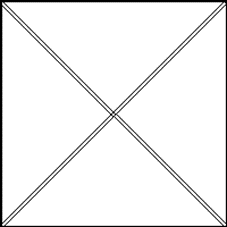
\includegraphics[width=150pt, keepaspectratio]{Imagens/FigA.png}
% % legenda da figura por baixo
% \caption{Exemplo de como considerar um gráfico}
% \label{fig:graficoecampl} % referência única da figura
% \end{figure}



% \section{Estatísticos\label{se:Estatísticos}}

% \section{Redes Neuronais\label{se:Redes Neuronais}}

% \subsection{Arquiteturas\label{sese:Arquiteturas}}


% \begin{table}[H]
% \caption{Resultados Arquiteturas}
% \resizebox{\linewidth}{!}{\input{/home/joao/Documentos/renewable-penetration/reports/DownwardUsedSecondaryReserveEnergy/downdata/archs_experiment/exp_result.tex}}        
% \end{table}


% \begin{table}[H]
% \caption{Resultados Arquiteturas}
% \resizebox{\linewidth}{!}{\input{/home/joao/Documentos/renewable-penetration/reports/DownwardUsedSecondaryReserveEnergy/downdata/archs_experiment/exp_result.tex}}        
% \end{table}


% \subsection{Loss\label{sese:Loss}}
% \subsubsection{Advance Loss functions\label{se:Advance_Loss_functions}}

% \begin{table}[H]
% \caption{Advance Loss functions}    
% \resizebox{\linewidth}{!}{\input{/home/joao/Documentos/renewable-penetration/reports/DownwardUsedSecondaryReserveEnergy/downdata/advance_losses_experiments/exp_result.tex}}        
% \end{table}


% \begin{table}[H]
% \caption{Advance Loss functions}
% \resizebox{\linewidth}{!}{\input{/home/joao/Documentos/renewable-penetration/reports/UpwardUsedSecondaryReserveEnergy/updata/advance_losses_experiments/exp_result.tex}}        
% \end{table}

% \subsubsection{Losses\label{se:Losses}}
% \begin{table}[H]
% \caption{Losses}
% \resizebox{\linewidth}{!}{\input{/home/joao/Documentos/renewable-penetration/reports/DownwardUsedSecondaryReserveEnergy/downdata/losses_experiments/exp_result.tex}}        
% \end{table}


% \begin{table}[H]
%     \caption{Losses}
%     \resizebox{\linewidth}{!}{\input{/home/joao/Documentos/renewable-penetration/reports/UpwardUsedSecondaryReserveEnergy/updata/losses_experiments/exp_result.tex}}        
%     \end{table}

% \subsection{Activations\label{se:Activations}}
% % \begin{table}[H]
% % \caption{Resultados Arquiteturas}
% % \resizebox{\linewidth}{!}{\input{/home/joao/Documentos/renewable-penetration/reports/DownwardUsedSecondaryReserveEnergy/downdata/activation_experiments/exp_result.tex}}        
% % \end{table}


% % \begin{table}[H]
% %     \caption{Resultados Arquiteturas}
% %     \resizebox{\linewidth}{!}{\input{/home/joao/Documentos/renewable-penetration/reports/UpwardUsedSecondaryReserveEnergy/updata/activation_experiments/exp_result.tex}}        
% %     \end{table}

% \subsection{Weights\label{se:Weights}}


% \subsubsection{Value\label{se:Value}}



% \begin{table}[H]
%     \caption{Resultados Arquiteturas}
%     \resizebox{\linewidth}{!}{\input{/home/joao/Documentos/renewable-penetration/reports/UpwardUsedSecondaryReserveEnergy/updata/weights_experiments/exp_result.tex}}        
%     \end{table}

% \subsubsection{Time\label{se:Time}}
% \begin{table}[H]
% \caption{Resultados Arquiteturas}
% \resizebox{\linewidth}{!}{\input{/home/joao/Documentos/renewable-penetration/reports/DownwardUsedSecondaryReserveEnergy/downdata/weights_experiments/exp_result.tex}}        
% \end{table}


% % \begin{table}[H]
% %     \caption{Resultados Arquiteturas}
% %     \resizebox{\linewidth}{!}{\input{/home/joao/Documentos/renewable-penetration/reports/UpwardUsedSecondaryReserveEnergy/updata/weights_experiment/exp_result.tex}}        
% %     \end{table}


\label{ch:resultados_discussao}
% Conclusões e sugestões futuras
\newpage
\thispagestyle{plain}
\chapter{Conclusões e sugestões futuras}

Primeiramente podemos ver pela análise estatistica\ref{tb:statitics_scores} e aplicando a ideia\cite{Elsayed}, simples modelos estatisticos conseguiriam resolver o problema em mãos, melhor do que o que é utilizado actualmente\ref{tb:benchmark_val}, e melhor do que muitos dos modelos profundos que testamos. \\
E se considerarmos ainda que os modelos estatiscos apresentados que apresentam estes resultados, utilizam apenas a variavel em questão, e não todos os outros atributos, a nível de aplicabilidade já são um melhoria. \\

Com modelos relativamente simples conseguimos melhorias muito grandes na alocaçao de energia, em relaçao à alocada actualmente. Este metodos podem criar ganhos fincanceiros grandes.



Aqui são dadas as respostas às perguntas de investigação formuladas na secção \ref{se:objetivos}. Não fazer aqui a discussão dos resultados. Essa discussão deve ser feita no capitulo \ref{ch:resultados_discussao}. Não esquecer de indicar sugestões futuras para que um colega possa dar continuidade ao trabalho desenvolvido. 


sintexe excutiva:

Os modelos de redes neuronais para previsões são um campo já bastante explorado. As varias gerações de arquiteturas sempre tentaram resolver este problema.


Como podemos verificar neste estudo esses metodos são mais eficazes que a técnica actualmente aplicada para a previsão de alocação secundária.

Uma primeira análise apenas linear já consegue resultados mais lucrativos que o modelo aplicado, então o poder das redes neuronais consegue ampliar essa capacidade.
Contudo a escolha e aplicação das mesmas deve estar fortemente ligado ao tipo de estrutura que se pretende construir para a mesma.
Em casos de grande capacidade computacional e previsões recorrentes os modelos de arquiteturas mais recente, e os modelos mais complexos, como UNET e a familia de Transformers, são os que mostram mais fiabilidade.
No entanto se estes calculos só podem ser efectuados em maquinas menos poderosas, pode-se ter de ficar pelos arquiteturas mais simples, e mais antigas (dar exemplos).

Independentemente do caso especifico, é bastante possivel melhorar o modelo actual de previsão usando redes neuronais, sendo que estas vao manter ainda a capacidade de ir aprendendo com dados novos, dando ainda mais robustez e dinamimo às previsões.


Embora os resultados sejam positivos do ponto de vista do problema a procurar ser resolvido, penso que poderia ser atacado de maneira mais eficaz.
Os primeiros passos para um modelo mais rebusto seria a escolha de dados de treino. Neste estudo usamos dados de outras previsões, dados esse que são eles proprios artificias na sua maioria. Isto não só adiciona mais uma camada de abstração, como representa uma perda na qualidade de informação.
Ao invés destes dados de previsões um primeiro passo seria criar um modelo apenas com dados reais de consumo e produção.
Em adicão a isto os principais dados a utilizar numa procura de melhor modelo seriam os de outras reservas, primária e terciária. Visto estas estarem intrincecamente ligadas com a reserva secundãria, deduzo que a informação contida nestes seria bem mais eficaz na produção de modelos de previsão de reserva de energia secundária.

Outra recomendação a ter em mente para futuros modelos requer já um conhecimento destes sistemas superior, e a criação de camadas neuronais com restrições na modelaçao das variaveis. Este tipo de camadas vai permitir modelos muito mais robustos, visto nao aprenderem fora do contexto necessário, e tambem modelos muito mais leves, o que irá permitir uma adopção dos mesmos mais eficaz.
\label{ch:conclusao}
% Referências Bibliográficas
\renewcommand{\bibname}{Referências} %comando para rename a BIBLIOGRAFIA para REFERENCIAS
\addcontentsline{toc}{chapter}{\numberline{10}Referências}
\printbibliography

% Referências Bibliográficas
\appendix
\newpage
\thispagestyle{plain}
\chapter{Anexos}

% Para introduzir figuras
\begin{figure}[H]
\centering
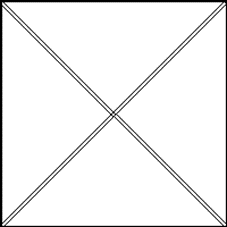
\includegraphics[width=150pt, keepaspectratio]{Imagens/FigA.png}
% legenda da figura por baixo
\caption{Exemplo de como considerar um gráfico nos anexos.}
\label{fig:grafico1} % referência única da figura
\end{figure}

\setlength\tabcolsep{4pt}
\begin{table}[H]
\centering
\caption{Isto é um exemplo de uma tabela. Se fôr igual(copiada) a outro autor deve ser pedido autorização para reproduzir.}
\begin{tabular}{p{5cm}p{3.5cm}p{2cm}p{2cm}}
\toprule %thicker line
\textbf{Title 1} & \textbf{Title 2} & \textbf{Title 3} & \textbf{Title 4} \\ \hline
\multirow{3}{*}{entry 1}   & data      & data    & data             \\
                           & data      & data    & data             \\
                           & data      & data    & data             \\ \hline
\multirow{2}{*}{entry 2}   & data      & data    & data             \\
                           & data      & data    & data             \\ \hline
\multirow{4}{*}{entry 3}   & data      & data    & data             \\
                           & data      & data    & data             \\
                           & data      & data    & data             \\
                           & data      & data    & data             \\ \hline
entry 4                    & data      & data    & data             \\ \hline 
\end{tabular}
\end{table}
\label{ch:Anexos}

\end{document}
